\documentclass{beamer}
% \documentclass[handout,xcolor=pdftex,dvipsnames,table]{beamer}
% \documentclass[draft]{beamer}
% \includeonlyframes{current,curr2}
\usepackage{enumerate}
\usepackage{hyperref}
\usepackage{amsmath}
\usepackage{amsthm}
\usepackage{amssymb}
\usepackage{amsfonts}
\usepackage{pdfpages}
\usepackage{booktabs}
\usepackage{nccmath}
\usepackage{bbm}

\usetheme{Boadilla}

\hypersetup{%
	pdftitle={Slides},%
	pdfauthor={James G. Partridge},%
	pdfsubject={},%
	pdfkeywords={Firm Capital, Credit Rating Agencies, Macro, School}%
}

\newtheorem{prop}[theorem]{Proposition}

\title[Information, Ratings and Corporate Bonds]{The Role of Public Information and Credit Ratings\\in the Corporate Bond Market}
\author[JGP]{James Partridge} 
\institute[UWO]{The University of Western Ontario}
\date[August 18, 2012]{Macro Lunch} 

\begin{document}

\begin{frame}[plain]%Title Page
\titlepage
\end{frame}

\begin{frame}{Credit Ratings}
\begin{itemize}
	\item 3 major credit rating agencies (CRAs)
	\begin{itemize}
		\item S\&P, Moody's, and Fitch (also Duff~\&~Phelps)
	\end{itemize}
	\item 3 major markets: sovereign/gov't, corporate, structured finance
	\begin{itemize}
		\item I focus on corporate bond ratings
	\end{itemize}
	\item The bond issuer pays for the rating
\end{itemize}
\end{frame}

\begin{frame}{Credit Ratings}
\begin{itemize}
	\item Rating system designed to measure relative credit risk
	\begin{itemize}
		\item Credit ratings are used as an aggregate measure of risk
	\end{itemize}
	\item AAA, AA, A \& BBB bonds considered investment grade (IG)
	\item BB, B, CCC, CC \& C bonds considered speculative grade (SG)
	\item Legal restrictions on ``institutional investors'' (e.g. pension funds) intended to limit risks in managed portfolios
\end{itemize}
\end{frame}

\begin{frame}{Puzzling Observation}
\begin{itemize}
	\item Number of AAA firms (S\&P): now 4, down from 34 in 1985!
	\item Number of AAA and AA rated firms have decreased, while the total number of firms with a rating has increased. 
\end{itemize}
\vspace{0.35cm}
\uncover<2->{
\hspace{0.8cm}\textbf{Question:} \\
\hspace{0.8cm}Why have so many high rated firms disappeared? \\
\vspace{0.5cm}
}
\uncover<3->{
\begin{quote}
Scores of big companies have lost their AAA status in recent years as it became seen in board rooms as more of a straitjacket than a path to riches.\\
\hspace*\fill \textup{\footnotesize{Eric Dash, New York Times, August 2, 2011}}
\end{quote}
}
\uncover<4->{
\hspace{0.8cm}\textbf{My conjecture:} \\
\begin{quote}
Ratings have value as a signal, but this value has diminished as information proliferation has increased.
\end{quote}
}
\end{frame}

{
\setbeamercolor{background canvas}{bg=}
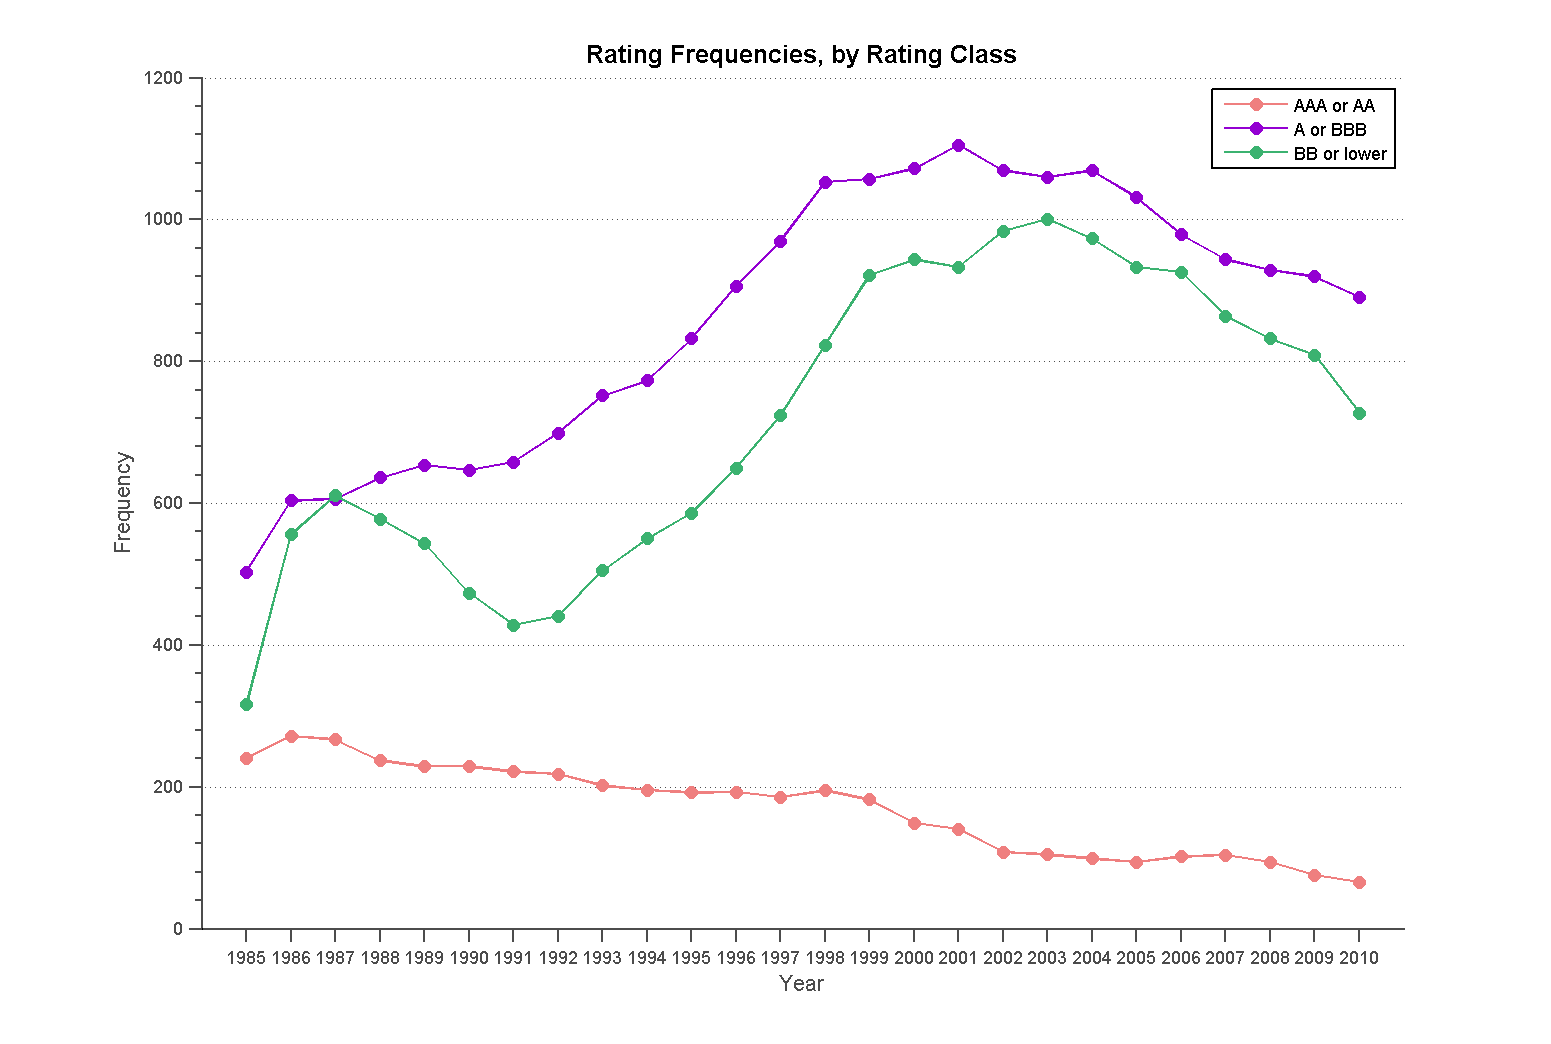
\includepdf{rate_freq.png}
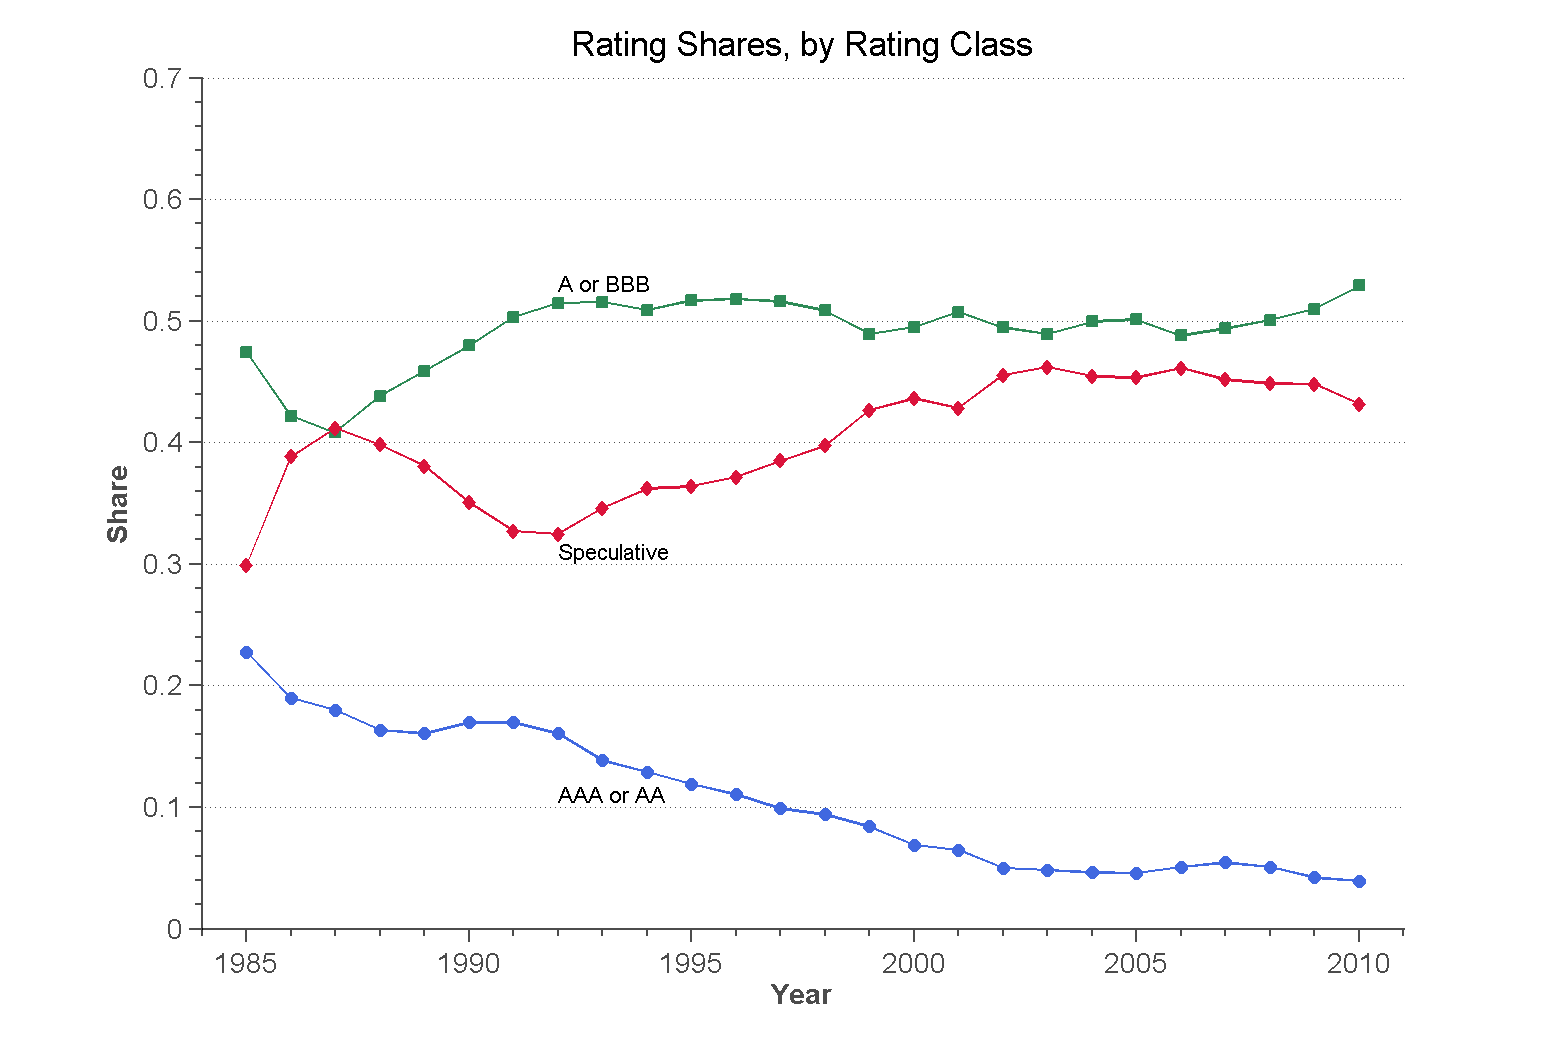
\includepdf{rate_share.png}
}

\begin{frame}{What I Do}
\begin{itemize}
	\item Show distribution of bond ratings has shifted away from high ratings
	\item Develop a model with credit ratings and public information to match this fact
	\item Test the following implication: price dispersion has increased for high-rated bonds
\end{itemize}
\end{frame}


\begin{frame}[label=robust]{The Fall of Highest Rated Firms is ``Robust''}
\begin{itemize}
	\item Not a question of evolving CRA standards/incentives
	\begin{itemize}
		\item leverage ratios are stable by rating
		\item leverage ratios are slightly higher by cohort
	\end{itemize}
	\hyperlink{app}{\beamergotobutton{Appendix}}
	\item These firms aren't simply merging
	\begin{itemize}
		\item ignoring the financial sector, the assets controlled by \\ AAA and AA firms have also decreased
	\end{itemize}
\end{itemize}
\begin{table}\centering
\small
\begin{tabular}{l *{6}r}
\toprule
  	& 1985  & 1990  & 1995  & 2000  & 2005  & 2010\\ \midrule
AAA  	& 34  	& 26  	& 17  	& 8  	& 4  	& 1\\
AA  	& 0  	& 4  	& 8  	& 3  	& 6  	& 8\\
A  	& 0  	& 1  	& 3  	& 9  	& 6  	& 7\\
BBB  	& 0  	& 0  	& 1  	& 2  	& 3  	& 3\\
B  	& 0  	& 1  	& 1  	& 0  	& 0  	& 0\\
Merged 	& 0  	& 1  	& 2  	& 6  	& 6  	& 6\\
Retired	& 0  	& 1  	& 2  	& 6  	& 9  	& 9\\ 
\bottomrule
\end{tabular}
\caption{Evolution of circa 1985 AAA firms}
\end{table}
\end{frame}

% \begin{frame}{Why Credit Ratings Matter}
% \begin{itemize}
	% \item There has been a shift from bank to bond and equity financing
	% \begin{itemize}
		% \item Bonds have doubled as a proportion of corporate liabilities
	% \end{itemize}
	% \item CRA standards seem to vary little over this period
	% \item Decline in AAA and AA not due to mergers
% \end{itemize}
% \hyperlink{liab_share}{\beamergotobutton{Appendix}}
% \end{frame}

\begin{frame}{Motivation}
\begin{itemize}
	\item There has been a shift from bank to bond and equity financing
	\begin{itemize}
		\item Bonds have doubled as a proportion of corporate liabilities
	\end{itemize}
	\item Policy changes vis-\`{a}-vis CRAs may not have intended effect
	\item CRAs have received much attention/criticism due to MBS and CDO ratings, but corporate bonds are a different product
	\item Financial press suggests three answers:
	\begin{itemize}
		\item investors in general have larger appetite for risk
		\item knowledgeable investors place less emphasis on CRA ratings
		\item firms now find it too costly to maintain high ratings
	\end{itemize}
	\item All three indicate that elite ratings now have a lower value
	\item What is the fundamental change?
\end{itemize}
\end{frame}


\begin{frame}{Story}
\begin{itemize}
	\item \alert<1>{Then:} CRA ratings were the primary source of firm information, few had access to SEC filings, firm prospectus,\ldots
	\item \alert<2>{Now:} Bloomberg, WSJ Online, etc. all provide market data and firm analysis; firm info is readily available
	\item Rating and third-party market analysis both act as signals of firm's well-being or quality
	\item Cost required to achieve high ratings
\end{itemize}
\begin{quote}
Investors now have direct information on firm quality -- \\ high quality firms no longer willing to incur cost of high ratings
\end{quote}
\end{frame}

{
\setbeamercolor{background canvas}{bg=}
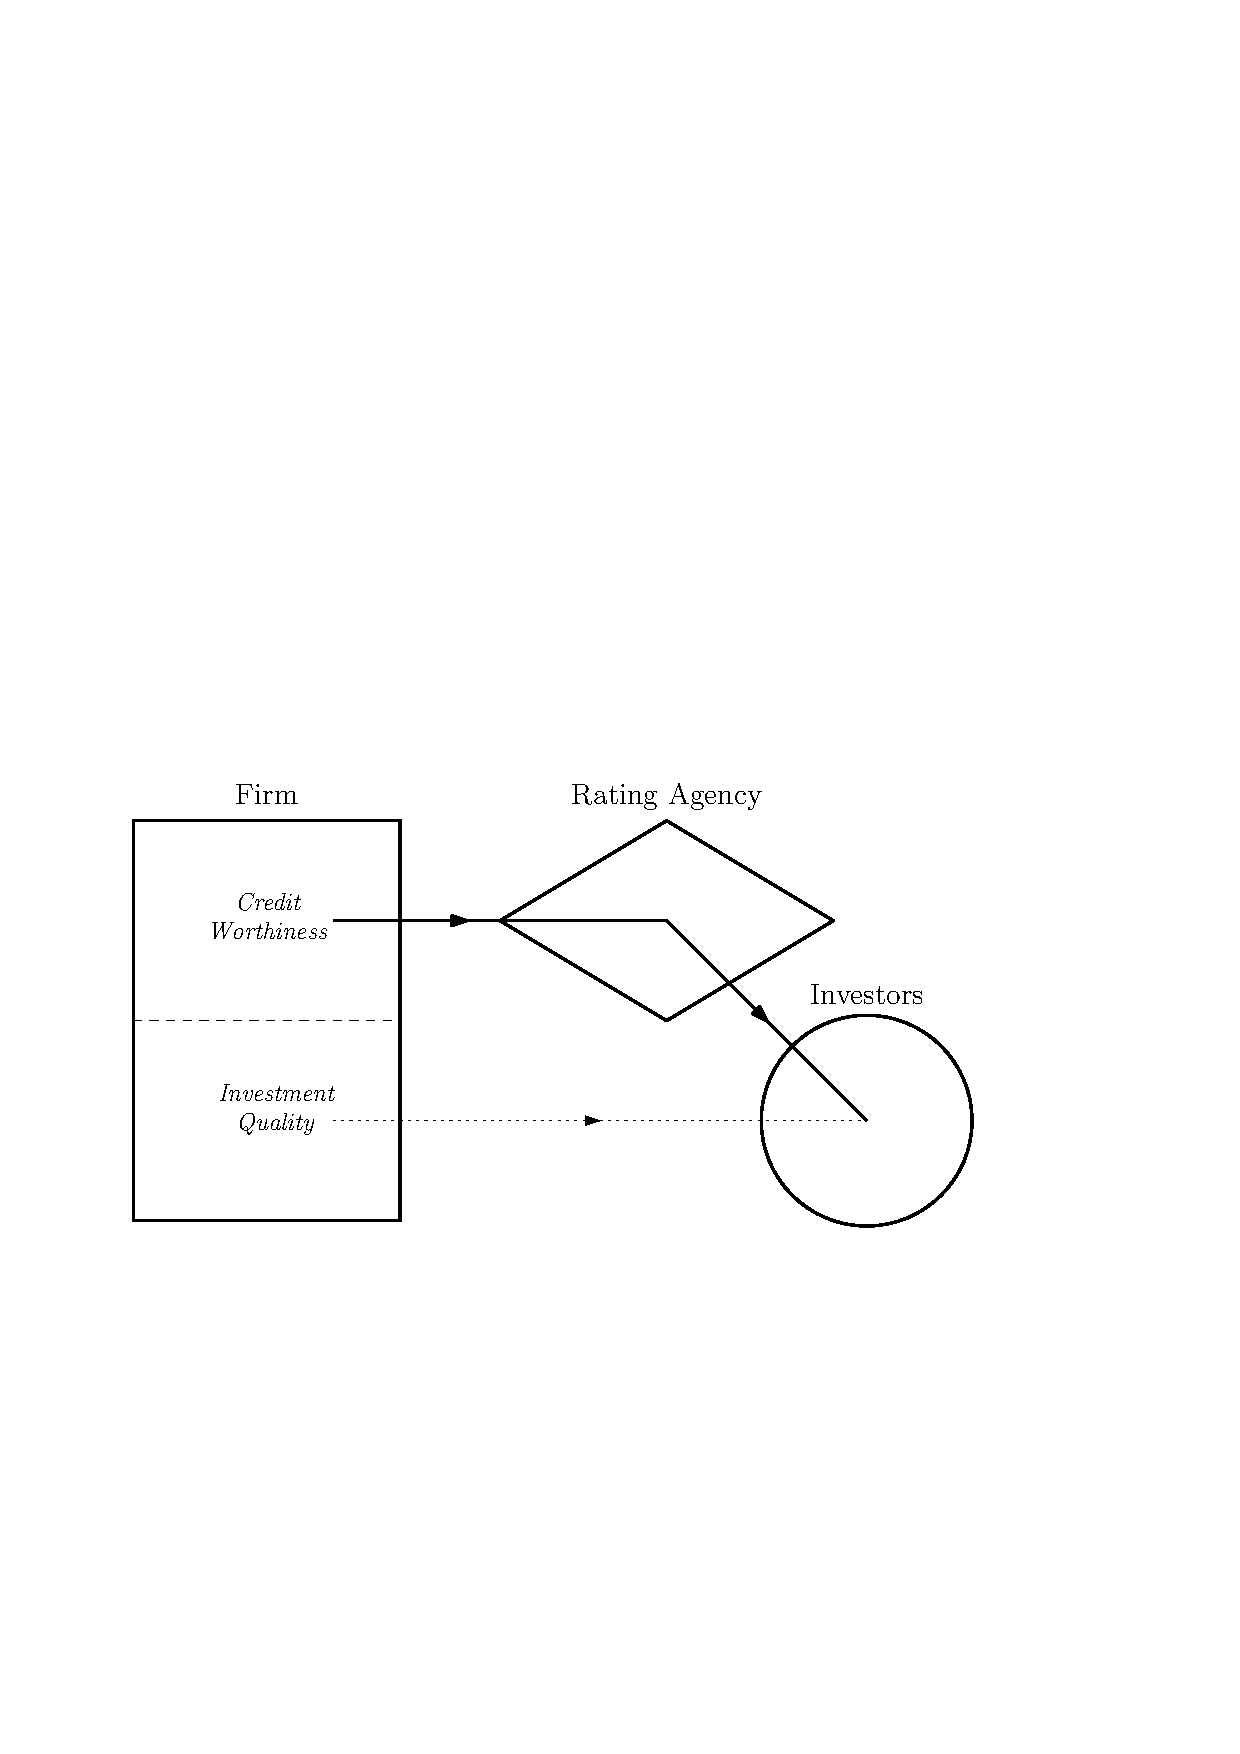
\includepdf{info_start}
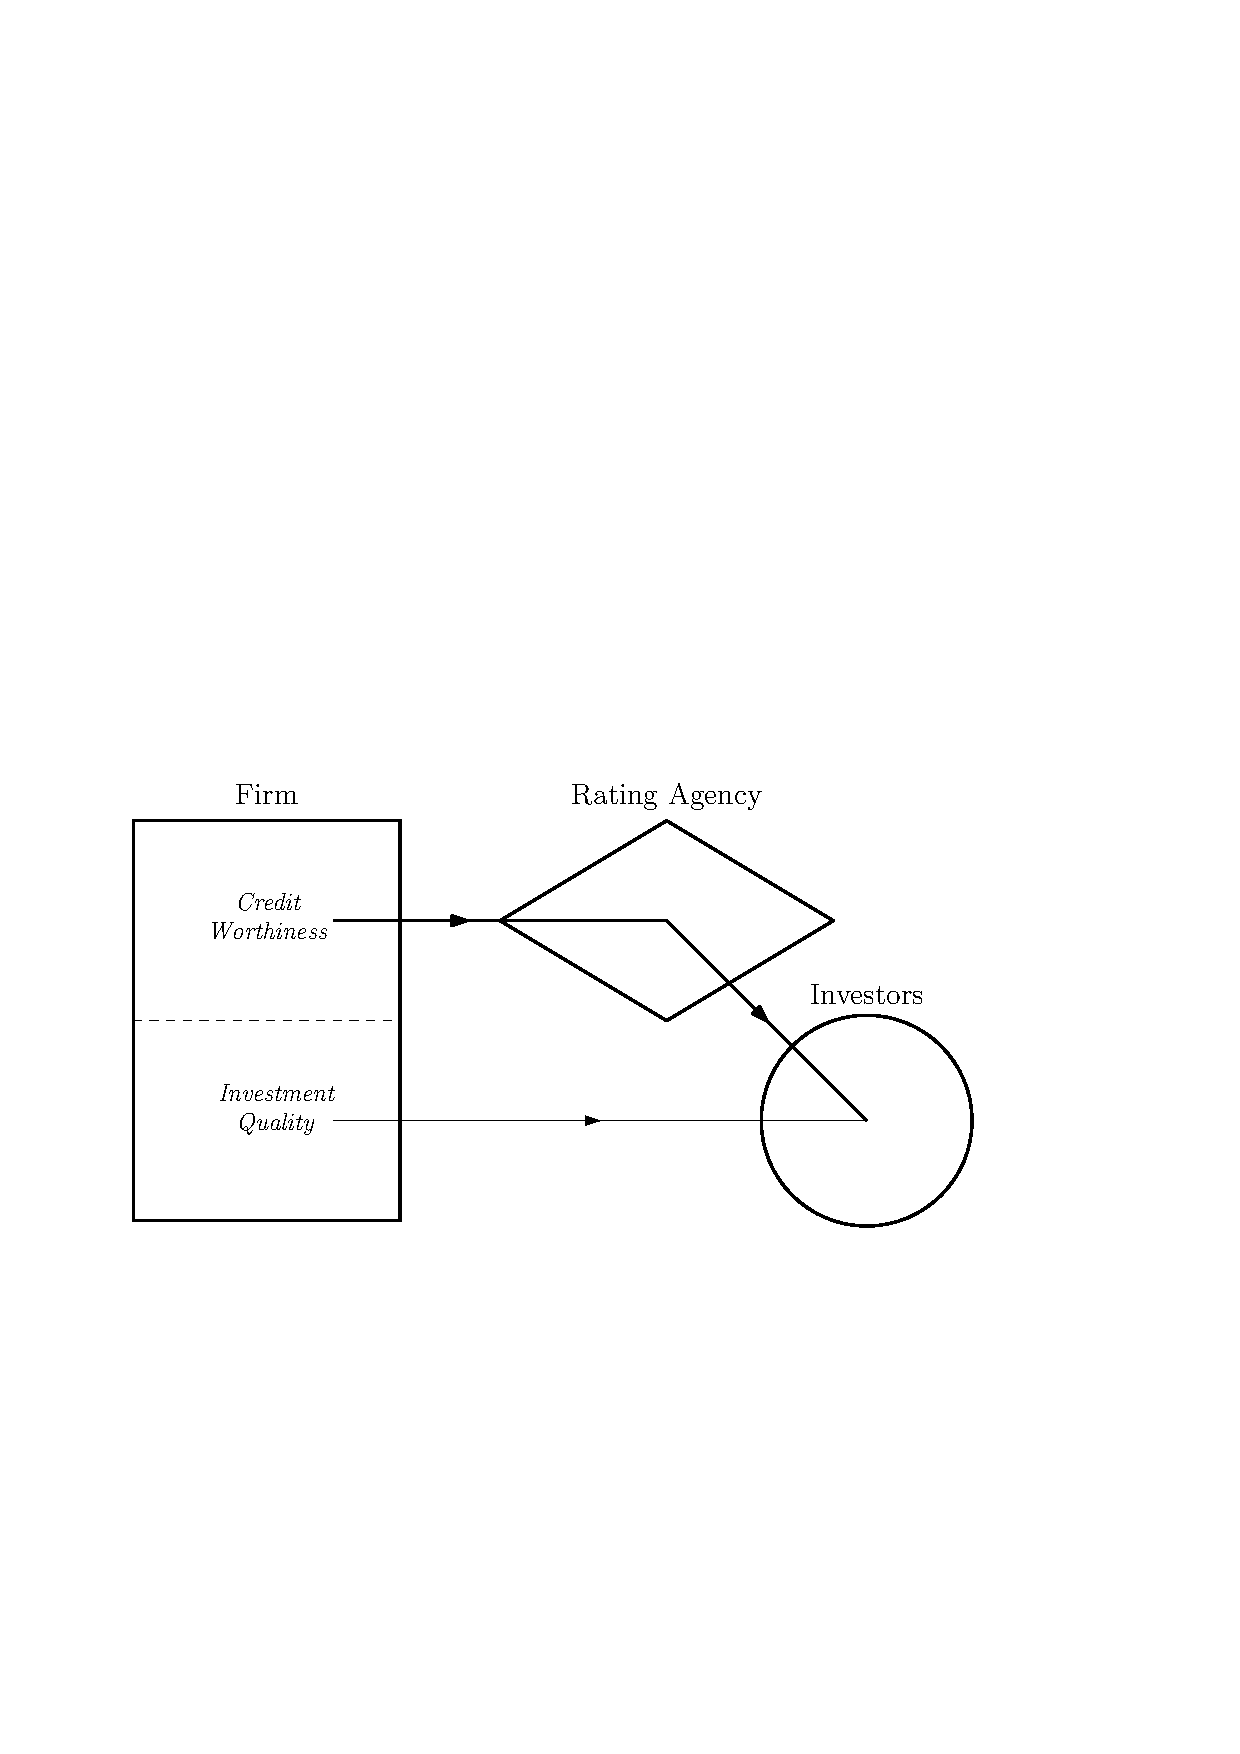
\includepdf{info_mid}
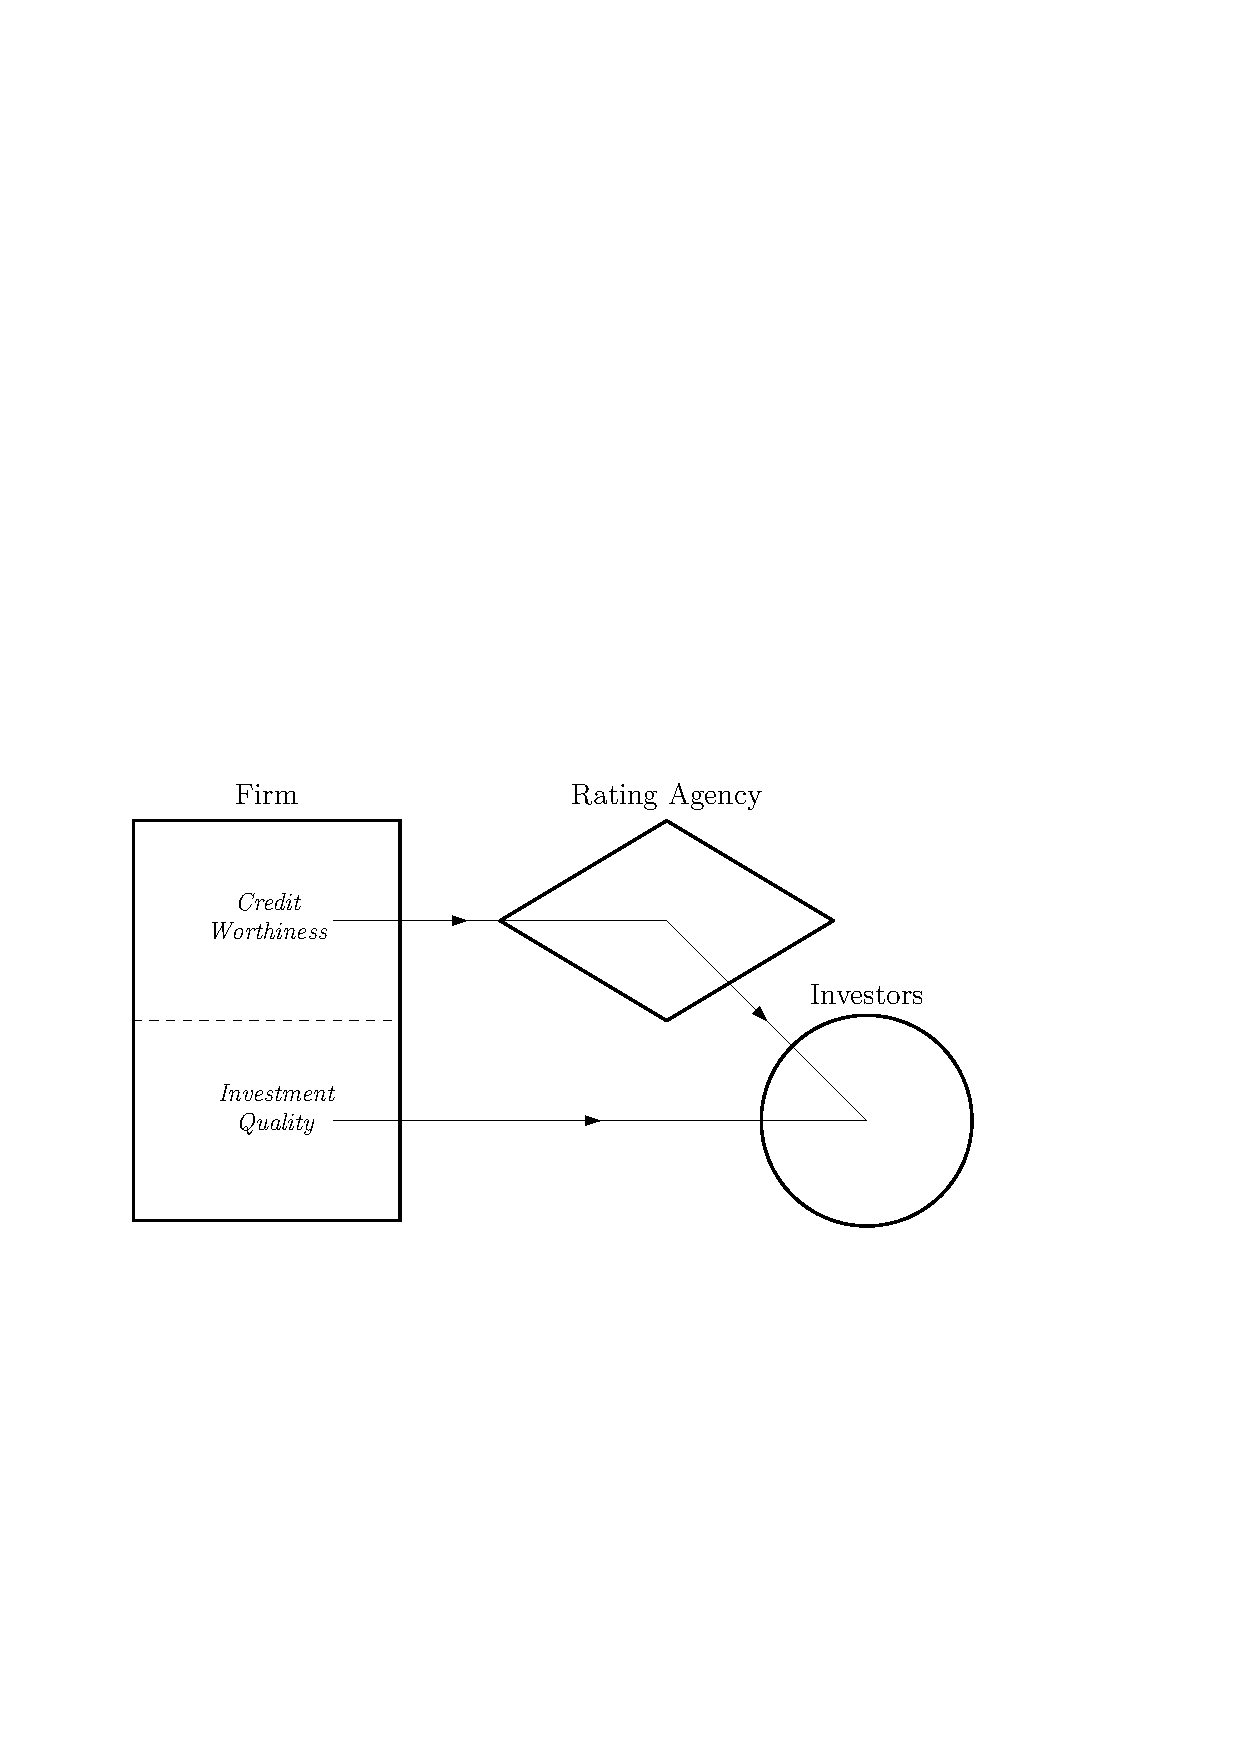
\includepdf{info_end}
}

\begin{frame}{Literature}
\begin{itemize}
	\item Academic literature has focused on other questions
	\begin{itemize}
		\item<1-> CRA incentives in structured finance market well-studied
		\alt<2>{
		\begin{itemize}
			\item Mathis, McAndrews \& Rochet 2009
			% \item Bar-Isaac \& Shapiro 2010
			\item Skreta \& Veldkamp 2009
			\item Bolton, Freixas \& Shapiro 2009
			\item He, Qian \& Strahan 2011
		\end{itemize}
		}{}
		\item<1-> feedback effects
		\alt<3>{
		\begin{itemize}
			\item Manso 2011
		\end{itemize}
		}{}
		\item<1-> bond, equity or bank financing
		\alt<4>{
		\begin{itemize}
			\item Bolton \& Freixas 2000
		\end{itemize}
		}{}
		% \item<1-> asymmetric info/credit rationing
		% \alt<5>{
		% \begin{itemize}
			% \item Stiglitz \& Weiss 1981
			% \item Bester 1985
		% \end{itemize}
		% }{}
		% \item<1-> decomposing spread over treasury
		% \alt<6>{
		% \begin{itemize}
			% \item Elton, Gruber, Agrawal \& Mann 2001
			% \item composed of risk, default, and tax premiums
		% \end{itemize}
		% }{}
		% sensitivity of bond prices to ratings change
	\end{itemize}
	\item Unique to this paper: firms influence their rating
\end{itemize}
\end{frame}

\begin{frame}{Environment}
\begin{itemize}
	\item Firms are of \textbf{type} $\theta \epsilon \left\{G,B\right\}$, unobserved by all
	\begin{itemize}
		\item determines probability the firm's project is successful
	\end{itemize}
	\item Economy receives a \textbf{signal}, $\nu$, about firm's type
	\begin{itemize}
		\item probability signal is `accurate' is $\omega$
		\item assume $\omega > 0.5$
	\end{itemize}
	\item The firm invests in the rating process, economy then observes \textbf{rating}
	\begin{itemize}
		\item accuracy of rating depends on investment
	\end{itemize}
\end{itemize}
\end{frame}

\begin{frame}{Timing}
\begin{enumerate}
	\item Ex ante:
	\begin{itemize}
		\item known: public signal ($H$ or $L$)
		\item unknown: type ($G$ or $B$)
	\end{itemize}
	\item Interim:
	\begin{itemize}
		\item firm chooses $\pi$
		\item rating is formed and observed ($A$, $B$ or $C$)
		\item debt contracts are issued, interest rates conditioned on $h$ and $\nu$
	\end{itemize}
	\item Ex post:
	\begin{itemize}
		\item outcome of project is realized (0 or $y$)
		\item debt is paid if project pays off
	\end{itemize}
\end{enumerate}
\end{frame}

\begin{frame}{Model}
\begin{itemize}
	\item Firms:
	\begin{itemize}
		\item endowed with a project that might earn $y$ if investment is received
		\item project requires investment $D$, fixed
		\item $\mathbbm{1}(h,\nu)=1$ if investment is received, 0 otherwise
	\end{itemize}
\end{itemize}
\begin{equation}
	\label{eq:FP}V(\nu)=\max_{\pi} \,\,\, -c(\pi)+\textup{E}_{\theta,h}\left [ \mathbbm{1}(h,\nu) \left (y - DR(h,\nu) \right )|\nu\right ]
\end{equation}
\begin{itemize}
	\item Investors:
	\begin{itemize}
		\item investors observe $\nu$ and $h$
		% \item choose whether to invest at $R(h,\nu)$
		\item have access to risk free outside option which pays $Dr$
		\item expected return is then:
	\end{itemize}
\end{itemize}
\begin{equation}
	\textup{E}_{\theta} \left [DR(h,\nu)|h,\nu \right ] = Dr
\end{equation}
\end{frame}

\begin{frame}{Distributions}
\begin{itemize}
\item Types:
	\begin{itemize}
	\item $Pr\left [\medmath{\theta=G}\right]=\lambda$
	\item $Pr\left [\medmath{\theta=B}\right]=1-\lambda$
	\end{itemize}
\item Ratings:
	\begin{itemize}
	\item $Pr\left [\medmath{h=A}|\medmath{\theta=G}\right ]=Pr\left [\medmath{h=C}|\medmath{\theta=B}\right ]=p_{1}+(p_{2}+p_{3})\pi$
	\item $Pr\left [\medmath{h=B}|\medmath{\theta=G}\right ]=Pr\left [\medmath{h=B}|\medmath{\theta=B}\right ]=p_{2}(1-\pi)$
	\item $Pr\left [\medmath{h=C}|\medmath{\theta=G}\right ]=Pr\left [\medmath{h=A}|\medmath{\theta=B}\right ]=p_{3}(1-\pi)$
	\end{itemize}
\item Signals:
	\begin{itemize}
	\item $Pr\left [\medmath{\nu=H}|\medmath{\theta=G}\right ]=Pr\left [\medmath{\nu=L}|\medmath{\theta=B}\right ]=\omega$
	\item $Pr\left [\medmath{\nu=L}|\medmath{\theta=G}\right ]=Pr\left [\medmath{\nu=H}|\medmath{\theta=B}\right ]=1-\omega$
	\end{itemize}
\end{itemize}
\end{frame}

\begin{frame}{Equilibrium}
\begin{block}{Definition}
An equilibrium is a set of interest rates, $\mathbf{R}^{*}=\left\{ R^{*}\left (h,\nu\right )\right\}_{h\epsilon\left\{A,B,C\right\}}^{\nu\epsilon\left\{H,L\right\}}$, and rating investment allocations, $\left\{\pi^{*}_{\nu}\right\}^{\nu\epsilon\left\{H,L\right\}}$ such that:
\begin{enumerate}
	\setlength{\itemindent}{0.8cm}
	\item given $\mathbf{R}^{*}$, $\pi^{*}_{\nu}$ maximizes $V(\nu)$;
	\item $\textup{E}_{\theta} \left [DR^{*}(h,\nu)|h,\nu \right ] = Dr \,\, \forall h, \nu$.
\end{enumerate}
\end{block}
\begin{itemize}
	\item Rational expectations implies $\pi^{*}$ is consistent with investor beliefs about $\pi$.
	\begin{itemize}
		\item Limit focus to interest rates that are mutually consistent, and consistent with $\pi^{*}$.
	\end{itemize}
\end{itemize}
\end{frame}

\begin{frame}{Equilibrium}
\begin{figure}
\centering
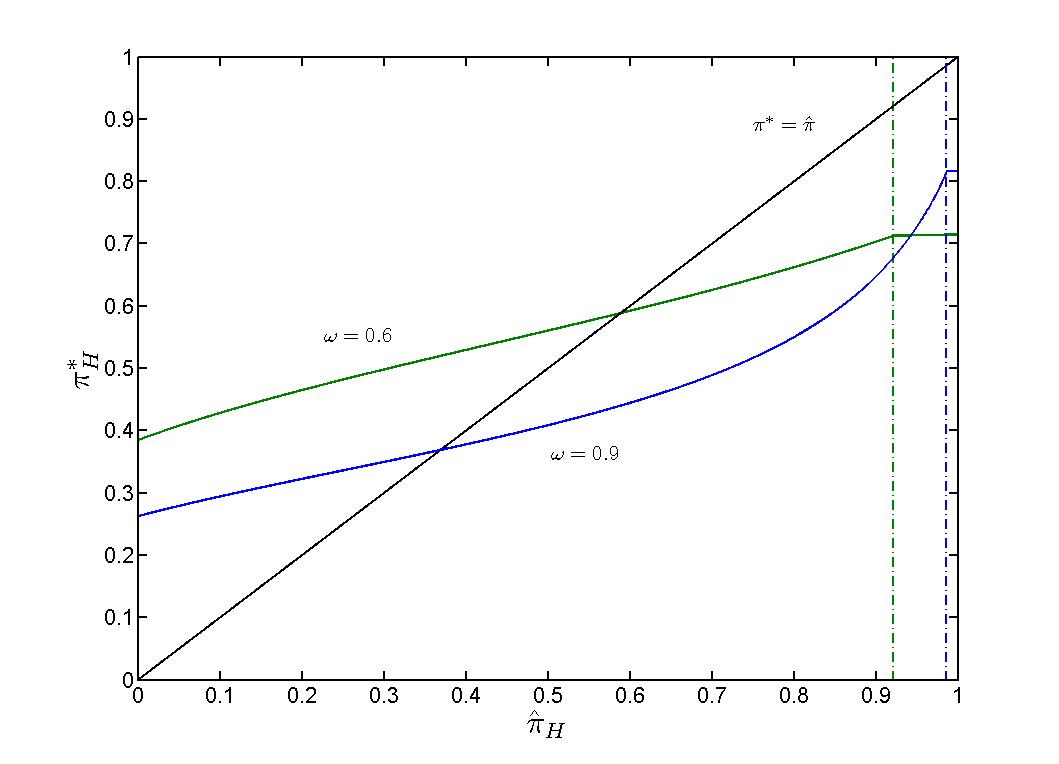
\includegraphics[width=0.8\textwidth]{EQ_comp_H_w.png}
\end{figure}
$\pi^{*}_{H}$ decreases as $\omega$ increases from 0.6 to 0.9.
\end{frame}

\begin{frame}{Equilibrium}
\begin{figure}
\centering
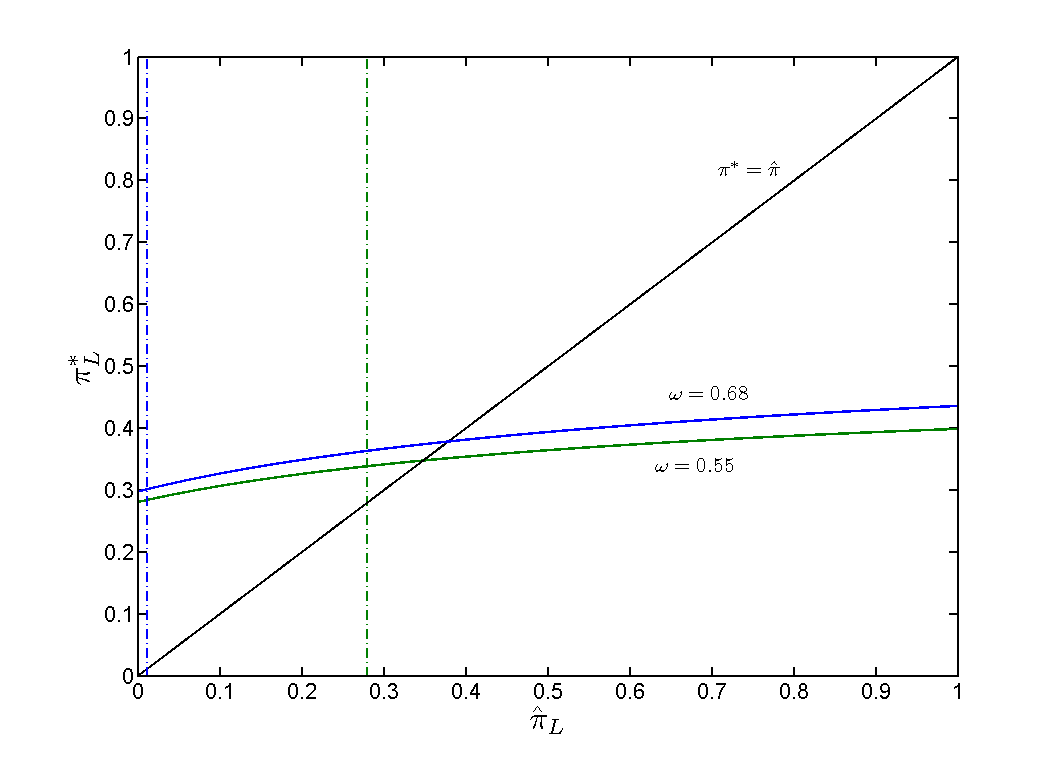
\includegraphics[width=0.8\textwidth]{EQ_comp_L_w.png}
\end{figure}
$\pi^{*}_{L}$ increases as $\omega$ increases from 0.55 to 0.68.
\end{frame}

\begin{frame}{Equilibrium}
\begin{figure}
\centering
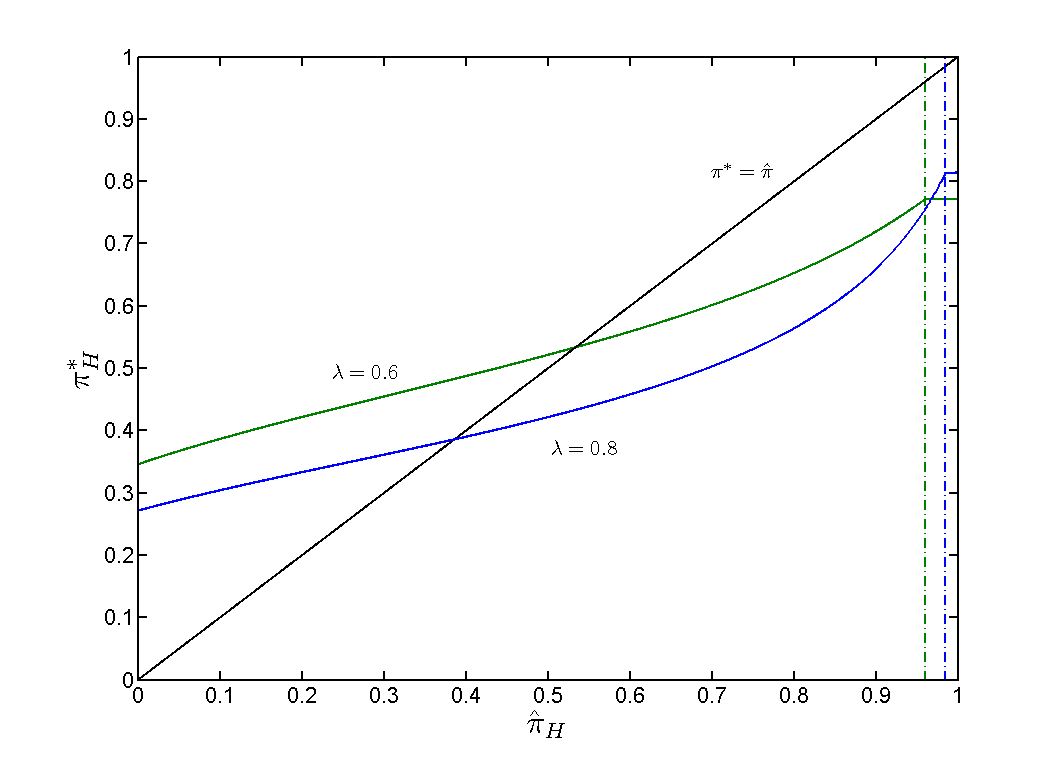
\includegraphics[width=0.8\textwidth]{EQ_comp_H_l.png}
\end{figure}
$\pi^{*}_{H}$ decreases as $\lambda$ increases from 0.6 to 0.8.
\end{frame}

\begin{frame}{Equilibrium}
\begin{figure}
\centering
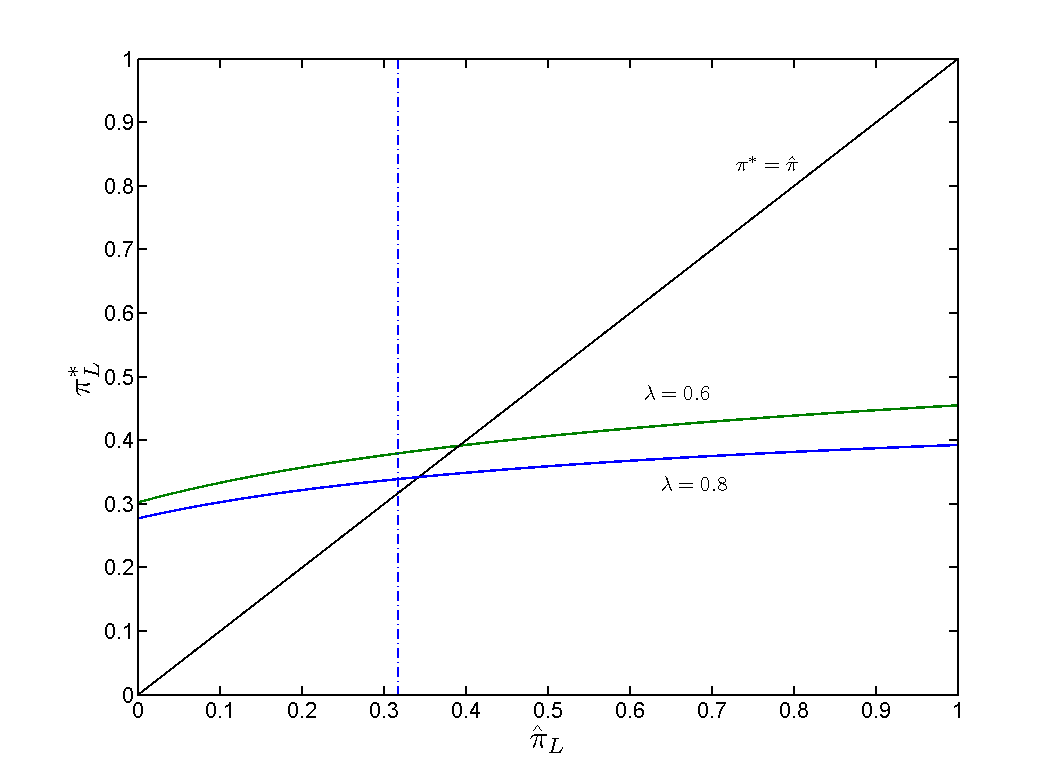
\includegraphics[width=0.8\textwidth]{EQ_comp_L_l.png}
\end{figure}
$\pi^{*}_{L}$ decreases as $\lambda$ increases from 0.6 to 0.8.
\end{frame}

%\begin{frame}{Equilibrium}
%Consider an investor who believes that $\left(\pi_{H},\pi_{L}\right)=\left(\hat{\pi}_{H},\hat{\pi}_{L}\right)$. Let $\mathbf{\hat{R}}$ be the interest rates that are consistent with this belief. 
%\begin{prop}
%In any equilibrium it must be the case that $\left(\hat{\pi}_{H},\hat{\pi}_{L}\right)=\left(\bar{\pi}_{H},\bar{\pi}_{L}\right)$.
%\end{prop}
%\begin{proof}
%Suppose not. Let $\left(\bar{\pi}_{H},\bar{\pi}_{L}\right)$ be the rating investment chosen by firms and $\bar{\mathbf{R}}$ be the implied interest rates. Suppose $\hat{\pi}_{\nu}<\bar{\pi}_{H}$. Then the expected return, $\textup{E}_{\theta} \left [D\hat{R}(H,\nu)|H,\nu \right ]$ is not equal to the 
%\end{proof}
%\end{frame}

\begin{frame}{Mechanism}
\begin{itemize}
	\item At certain interest rates $y-DR(h,\nu)<0$ so firms cannot commit to honour debt
	\item Implies firms that are (almost) known to be type $B$ will not get an investment
	\item Firms weigh benefit of lower borrowing cost against increasing cost of $\pi$ knowing they might be lowering the probability of investment if they are a $B$ type
	\item As $\omega$ increases correlation between signal and type increases, thus firms (and investors) learn more about their type
\end{itemize}
\end{frame}

\begin{frame}{Result}
\begin{prop}
There exists some $\bar{\omega}$ such that $\pi^{*}_H$ is decreasing in $\omega$ $\forall \omega > \bar{\omega}$.
\end{prop}
\begin{itemize}
	\item As $\omega$ increases, all firms choose lower $\pi$
	\begin{itemize}
		\item leads to less $A$, more $B$ ratings
	\end{itemize}
	\item Interest rate spread increases for firms with different signal, same rating
	\begin{itemize}
		\item testable implication
	\end{itemize}
\end{itemize}
\end{frame}

{
\setbeamercolor{background canvas}{bg=}
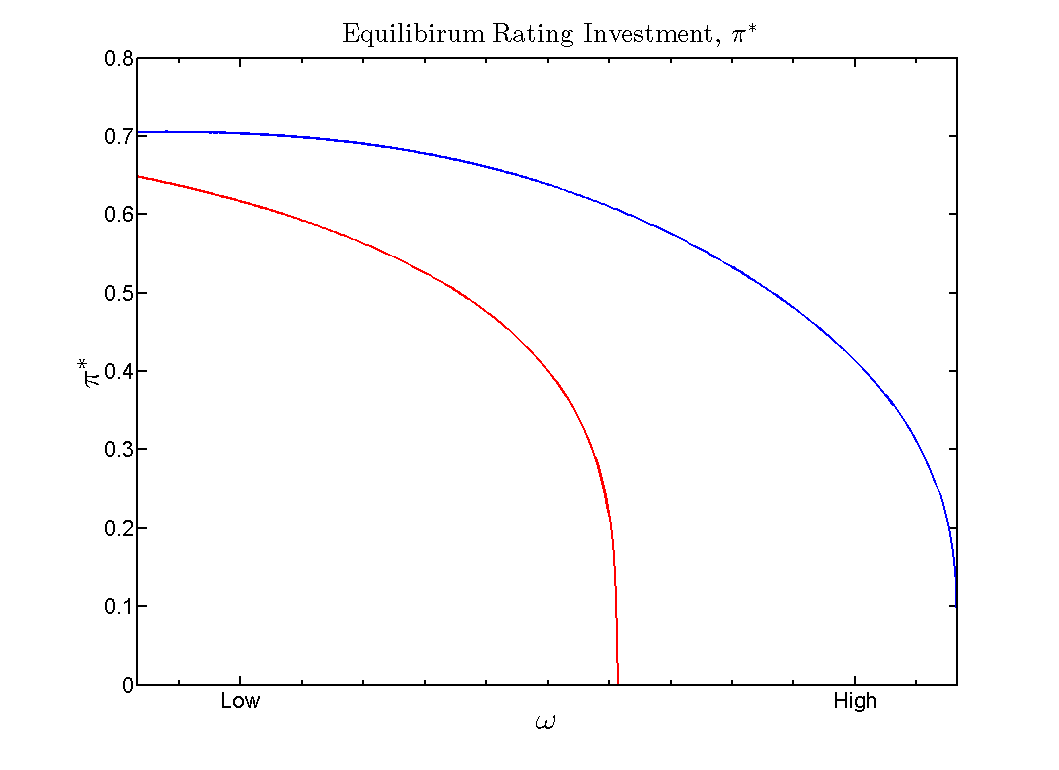
\includepdf{eq_inv.png}
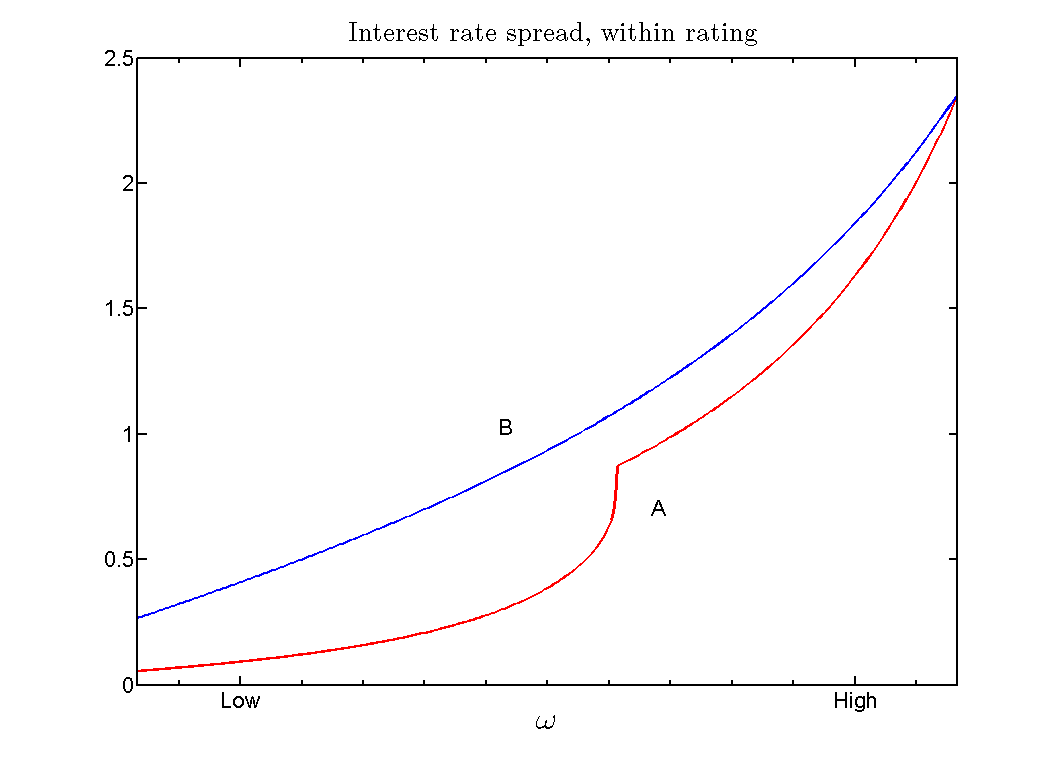
\includepdf{spreads.png}
}

\begin{frame}{Data}
Mergent Fixed Income Securities Database
\begin{itemize}
	\item All of the information is sourced from prospectuses
	\item For CUSIP and ratings data, Mergent obtains direct feeds
	\item Has ratings from the 4 major agencies
	% \item Also reports the reason for a rating change
\end{itemize}
\end{frame}

\begin{frame}{Data}
\begin{itemize}
	\item 4 year bins starting in 1990, ending 2009
	\item Use yield to maturity spread over treasury bonds at offering
	\begin{itemize}
		\item Captures the risk/default premium paid by firms 
	\end{itemize}
	\item Keep only fixed coupon bonds (90-100\% in every year)
	\item Use the rating closest to offering
	\begin{itemize}
		\item 80\% within 2 days of offering, 80\% before offering
	\end{itemize}
	% \item Break ties by taking the maximum rating
	% \item Drop financials and utilities
	\item 8,755 offerings
\end{itemize}
\end{frame}

%Table of observation frequencies
\begin{frame}{Data}
\begin{table}\centering
\begin{tabular}{l *{6}r}
\toprule
Ratings & 1990-1993 & 1994-1997 & 1998-2001 & 2002-2005 & 2006-2009 & Total\\ \midrule
All & 1080 & 1624 & 2422 & 2071 & 1551 & 8748\\
AAA/AA & 223 & 228 & 287 & 134 & 91 & 963\\ 
A/BBB & 719 & 980 & 1346 & 866 & 902 & 4813\\ 
SG & 138 & 416 & 789 & 1071 & 558 & 2972\\ 
\bottomrule
\end{tabular}
\caption{Observations in each rating-period bin}
\end{table}
\end{frame}

\begin{frame}{Data}
\begin{table}\centering
\begin{tabular}{l *{6}r}
\toprule
Ratings & 1990-1993 & 1994-1997 & 1998-2001 & 2002-2005 & 2006-2009 & Total\\ \midrule
All & 410 & 769 & 1205 & 1208 & 736 & 4328\\
AAA/AA & 77 & 65 & 111 & 57 & 30 & 340\\
A/BBB & 271 & 396 & 560 & 397 & 325 & 1949\\
SG & 69 & 332 & 583 & 783 & 408 & 2175\\
\bottomrule
\end{tabular}
\caption{Number of firms issuing debt in each rating-period bin}
\end{table}
\end{frame}

\begin{frame}{Bond Types}

\begin{table}[htbp]\centering 
\begin{tabular} {@{} l *{6}r @{}} \\ \toprule
 & \multicolumn{2}{c}{1990-2009} & \multicolumn{2}{c}{1990-1999} & \multicolumn{2}{c}{2000-2009} \\
 \cmidrule(r){2-3} \cmidrule(r){4-5} \cmidrule(r){6-7}
Type  & \# & \% & \# & \% & \# & \% \\ \midrule
CCOV  & 2     & 0.02  & 2     & 0.05    & 0     &  \\ 
CCUR  & 284   & 3.24  & 56    & 1.38    & 228   & 4.86\\ 
CDEB  & 7,625 & 87.09 & 3,520 & 87.00   & 4,105 & 87.47\\ 
CMTN  & 217   & 2.48  & 127   & 3.13    & 90    & 1.92\\ 
CPAS  & 391   & 4.47  & 312   & 7.68    & 79    & 1.68\\ 
CPIK  & 24    & 0.27  & 1     & 0.02    & 23    & 0.49\\ 
EBON  & 193   & 2.20  & 26    & 0.64    & 167   & 3.56\\ 
PS    & 6     & 0.07  & 6     & 0.15    & 0     &  \\ 
PSTK  & 5     & 0.06  & 5     & 0.12    & 0     &  \\ 
TPCS  & 7     & 0.08  & 7     & 0.17    & 0     &  \\ 
UCID  & 1     & 0.01  & 0     &         & 1     & 0.02\\ \midrule
Total & 8,755 &       & 4,062 &         & 4,693 & \\ 
\bottomrule
\end{tabular}
\end{table}
\end{frame}


\begin{frame}{Price Dispersion}
\begin{itemize}
	\item As information proliferates bond prices are affected
	\begin{itemize}
		\item Investors condition on ratings \textit{and} public information
	\end{itemize}
	\item Standard deviation of bond prices increasing for each rating class...
	\begin{itemize}
		\item but so is the mean...
		\item so use coeffecient of variation (CV) instead
	\end{itemize}
	\item Can test for statistical significance
	% \begin{itemize}
		% \item Need assumption of log-normality
	% \end{itemize}
\end{itemize}
\end{frame}

{
\setbeamercolor{background canvas}{bg=}
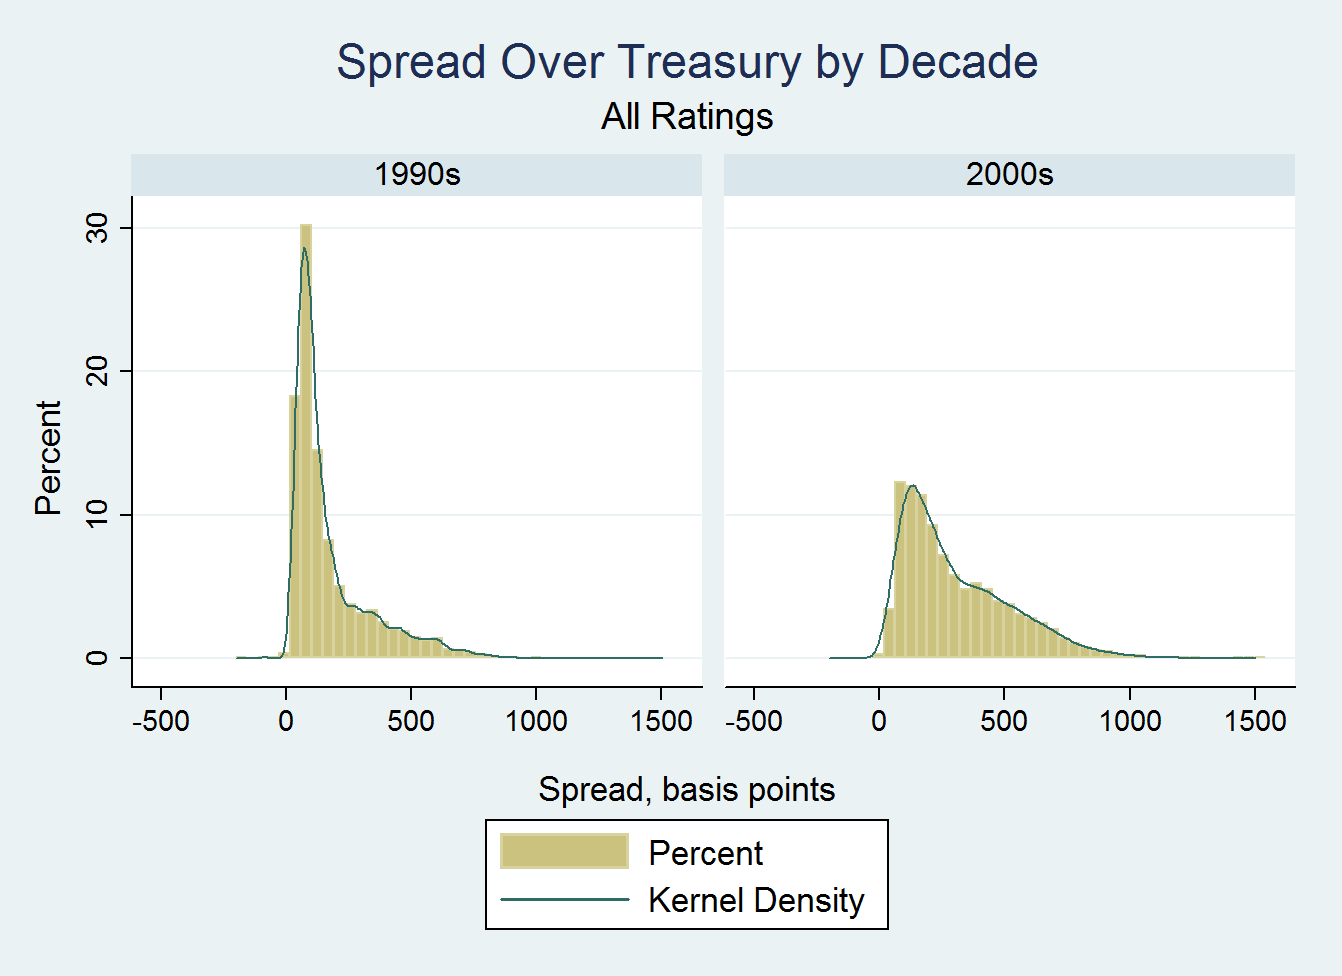
\includepdf{SpreadAll.png}
}
{
\setbeamercolor{background canvas}{bg=}
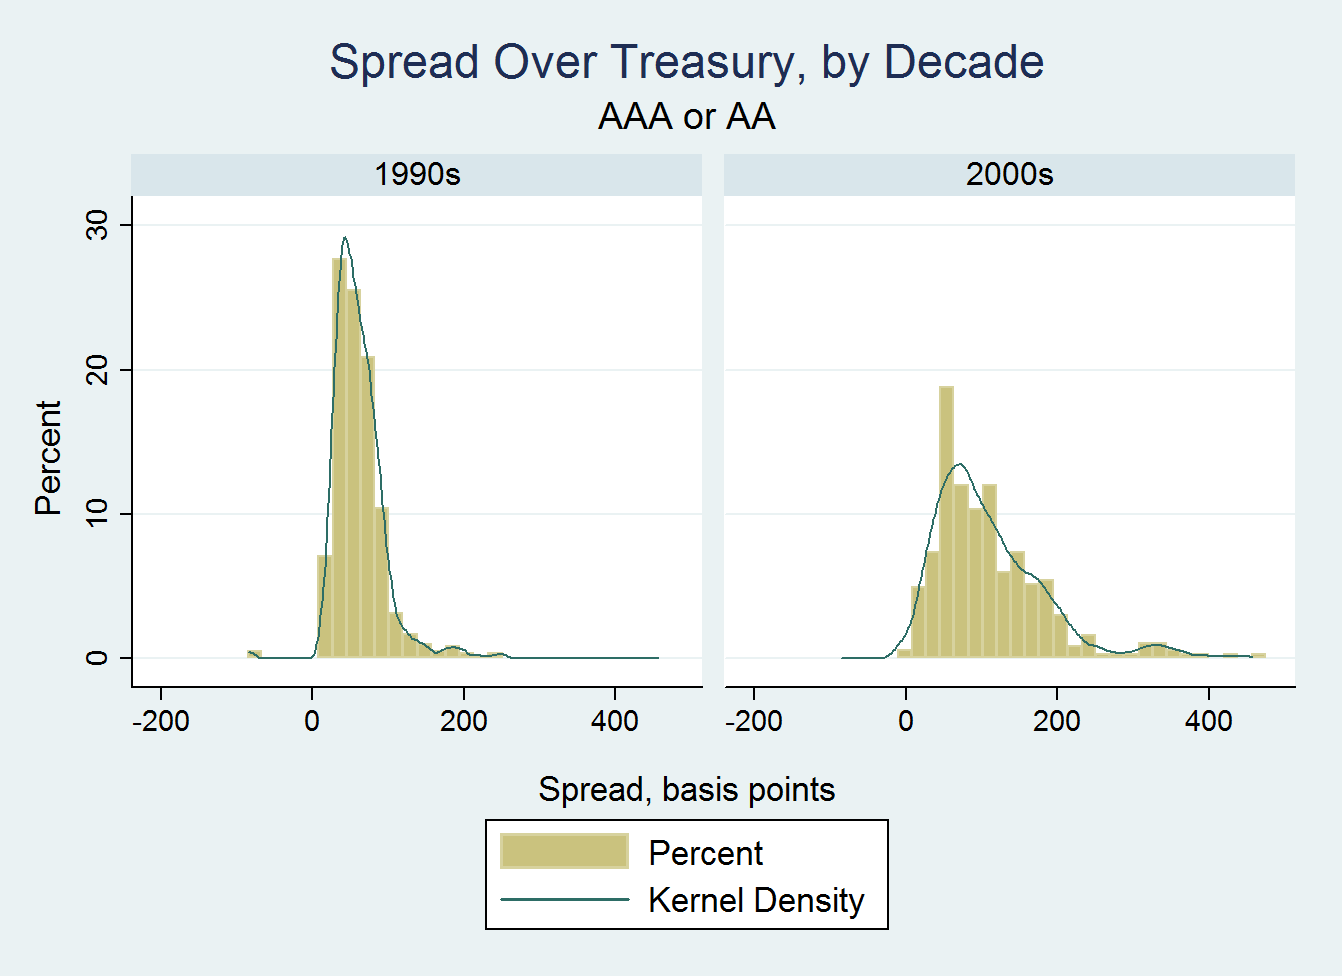
\includepdf{Spread_HiIG.png}
}
{
\setbeamercolor{background canvas}{bg=}
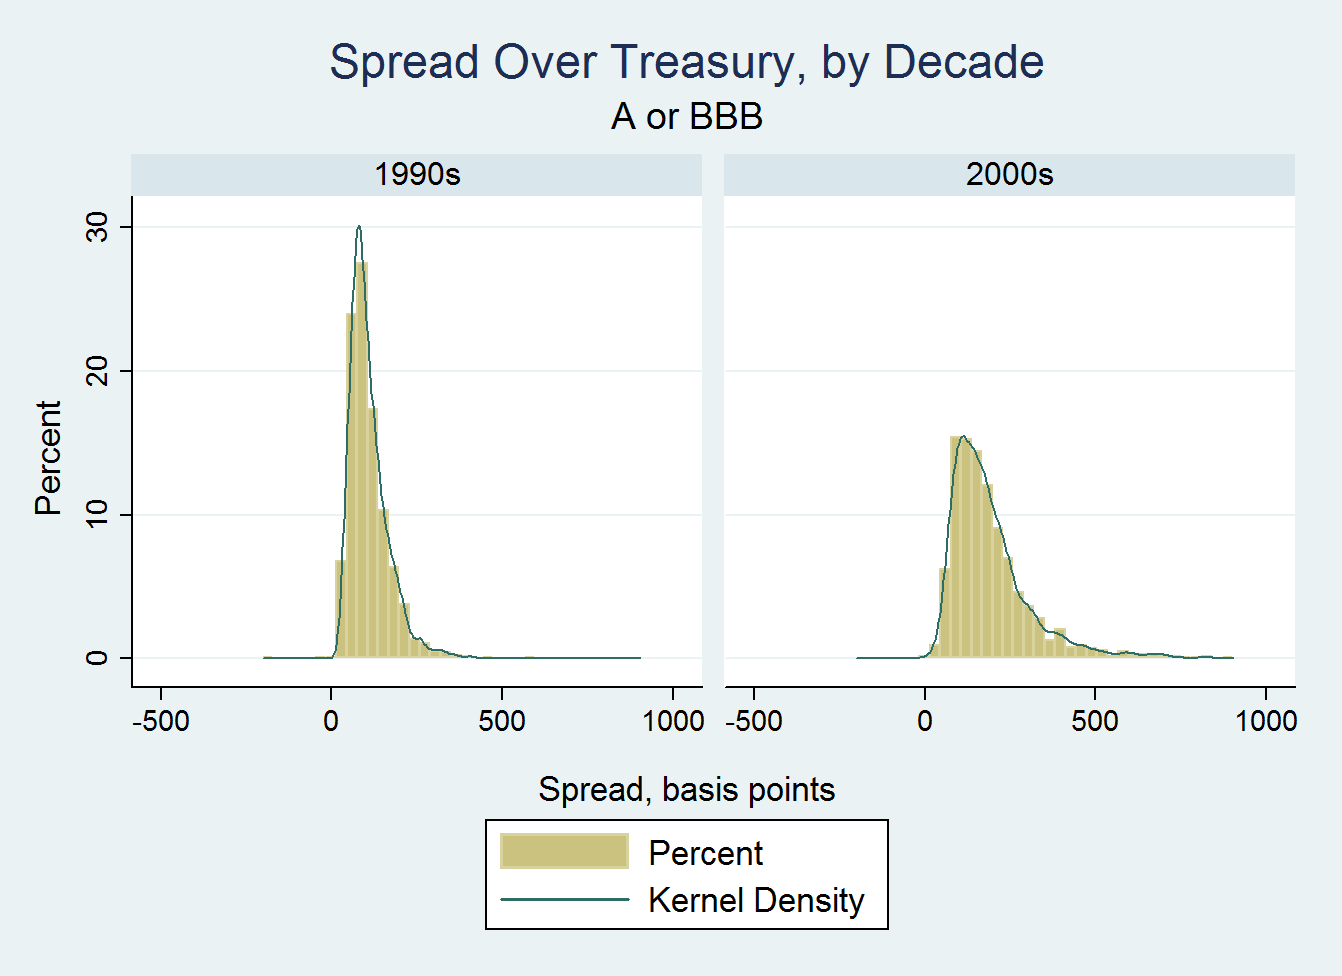
\includepdf{Spread_LoIG.png}
}
% {
% \setbeamercolor{background canvas}{bg=}
% 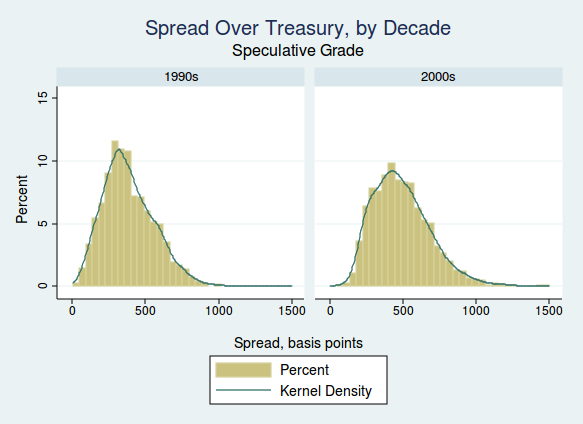
\includepdf{Spread_SG.png}
% }
% {
% \setbeamercolor{background canvas}{bg=}
% 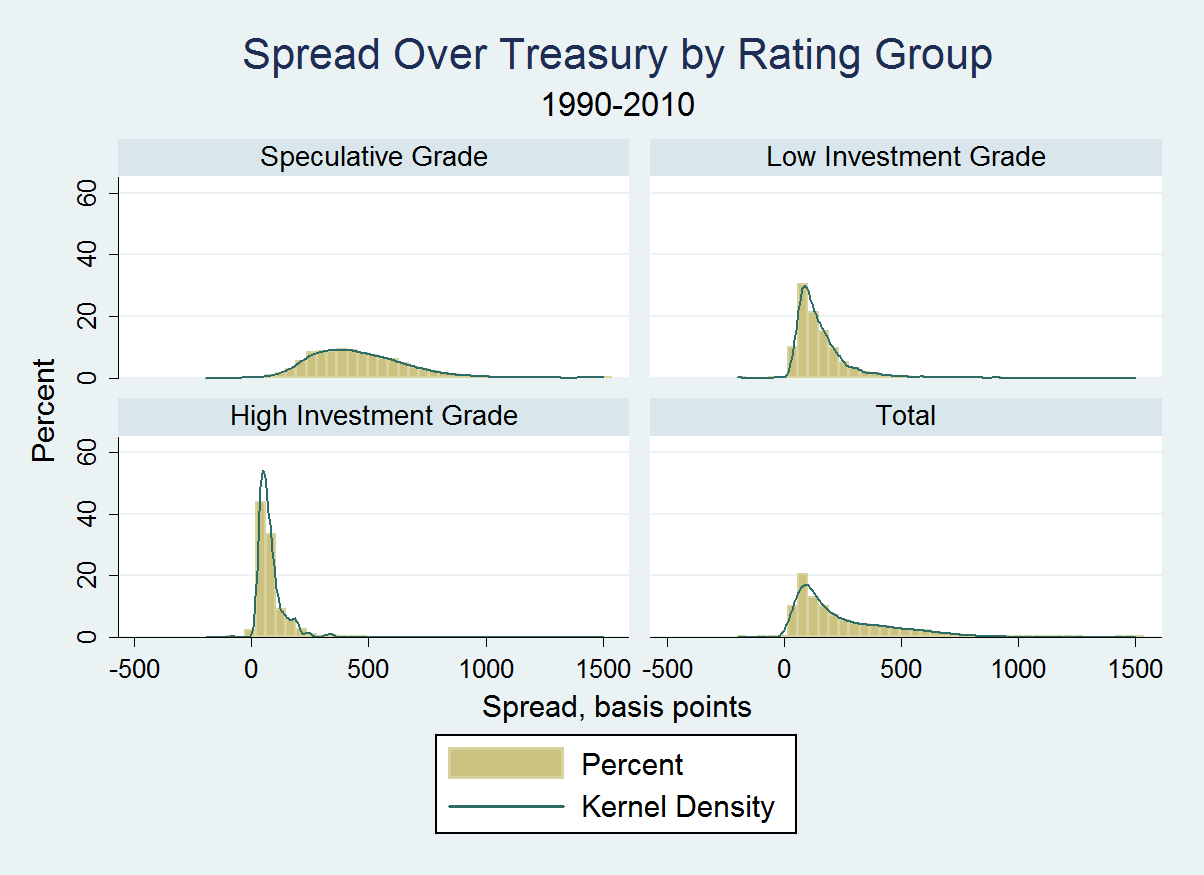
\includepdf{Spread_grp.png}
% }

{
\setbeamercolor{background canvas}{bg=}
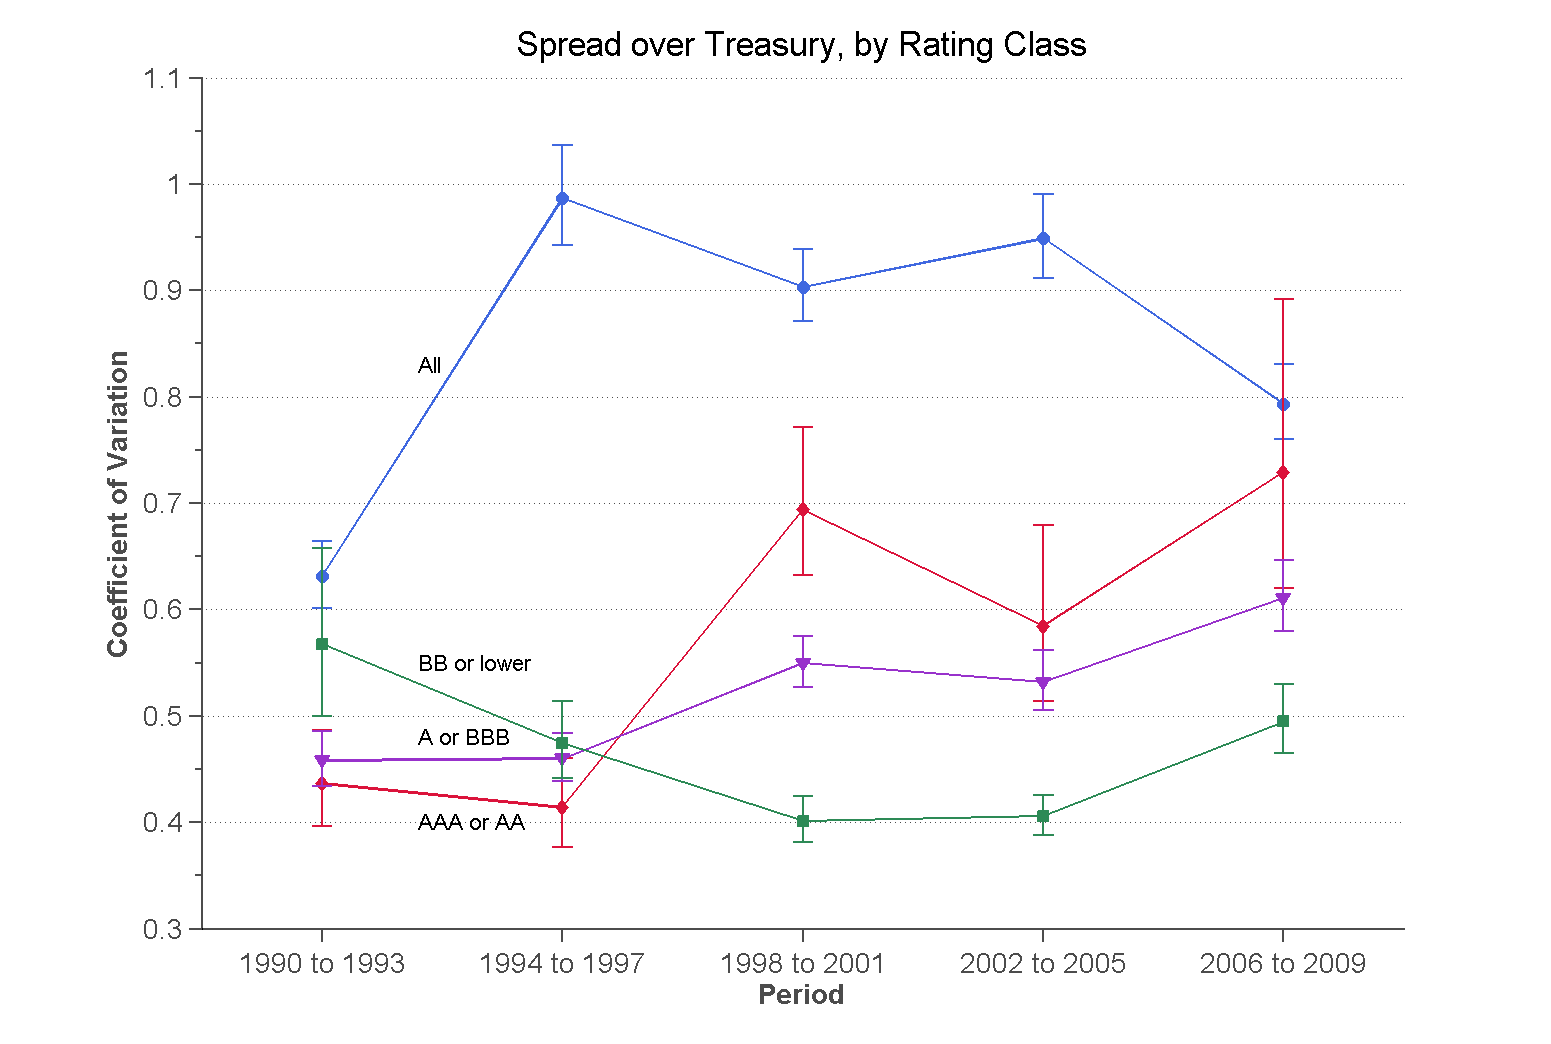
\includepdf{CVCI.png}
}

% \begin{frame}{Alternative Story}
% \begin{itemize}
	% \item Treasury rate has decreased
	% \item 1990s: 6\%
	% \item 2000s: 4\%
% \end{itemize}
% \end{frame}

% \begin{frame}{Agenda}
% \begin{itemize}
% 	\item Model
% 	\begin{enumerate}
% 		\item 2 types of investors: institutional and other
% 		%\item investor appetite for risk
% 		\item adverse selection: firms observe their type
% 		%\item recovery rate, leverage ratios
% 	\end{enumerate}
% 	\item Extensive and intensive margin: 
% 	\begin{itemize}
% 		\item large changes in issues per firm, firms per period
% 	\end{itemize}
% 	\item Behaviour of the SG bonds
% 	\begin{itemize}
% 		\item price dispersion
% 		\item frequency
% 	\end{itemize}
% \end{itemize}
% \end{frame}

\begin{frame}{Conclusion}
\begin{itemize}
	\item Vanishing AAAs consistent with improved information about firm quality
	\item Story implies an increase in bond price dispersion
	\item Consistent with new data:
	\begin{enumerate}
		\item distribution of bond ratings has shifted away from high ratings
		\item price dispersion has increased within rating
	\end{enumerate}
	\item Changes in rating distribution aren't necessarily caused by changing CRA standards
% 	\item Social efficiency...
\end{itemize}
\end{frame}

\begin{frame}[label=app]{Appendix}
\addtocounter{framenumber}{-1}
\begin{itemize}
\item Leverage ratios\\
\hyperlink{lev_rating}{\beamergotobutton{By Rating}} \hyperlink{lev_cohort}{\beamergotobutton{By Cohort}}
\item Assets\\
\hyperlink{assets}{\beamergotobutton{Assets}}
\item Numbers dropping in every cohort of AAA and AA\\
\hyperlink{cohorts}{\beamergotobutton{Cohorts}}
\end{itemize}
\hyperlink{robust}{\beamergotobutton{Back}}
\end{frame}

\frame[plain,label=lev_rating]{
\addtocounter{framenumber}{-1}
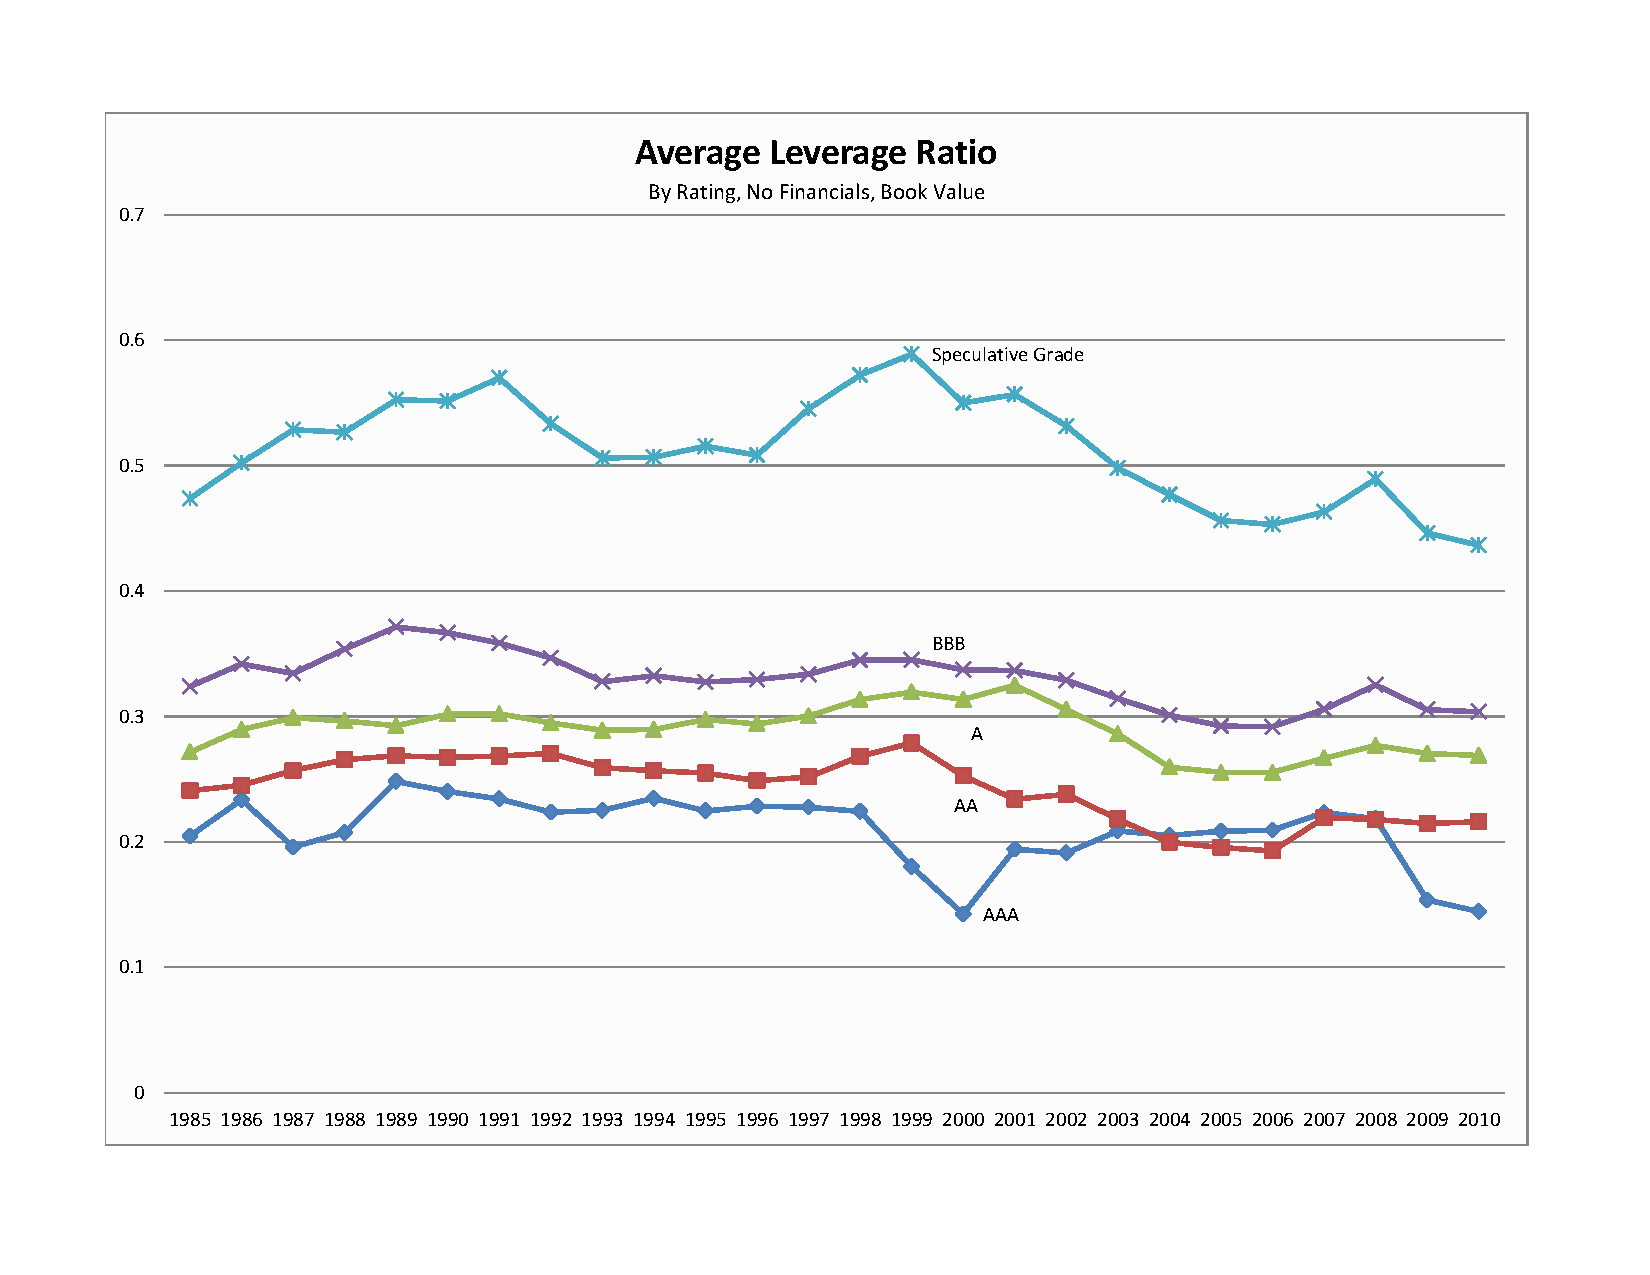
\includegraphics[page=1,width=\textwidth]{avg_leverage_bv_nofin.pdf}
\hspace{-11cm}\hyperlink{app}{\beamergotobutton{Back}}}

\frame[plain,label=lev_cohort]{
\addtocounter{framenumber}{-1}
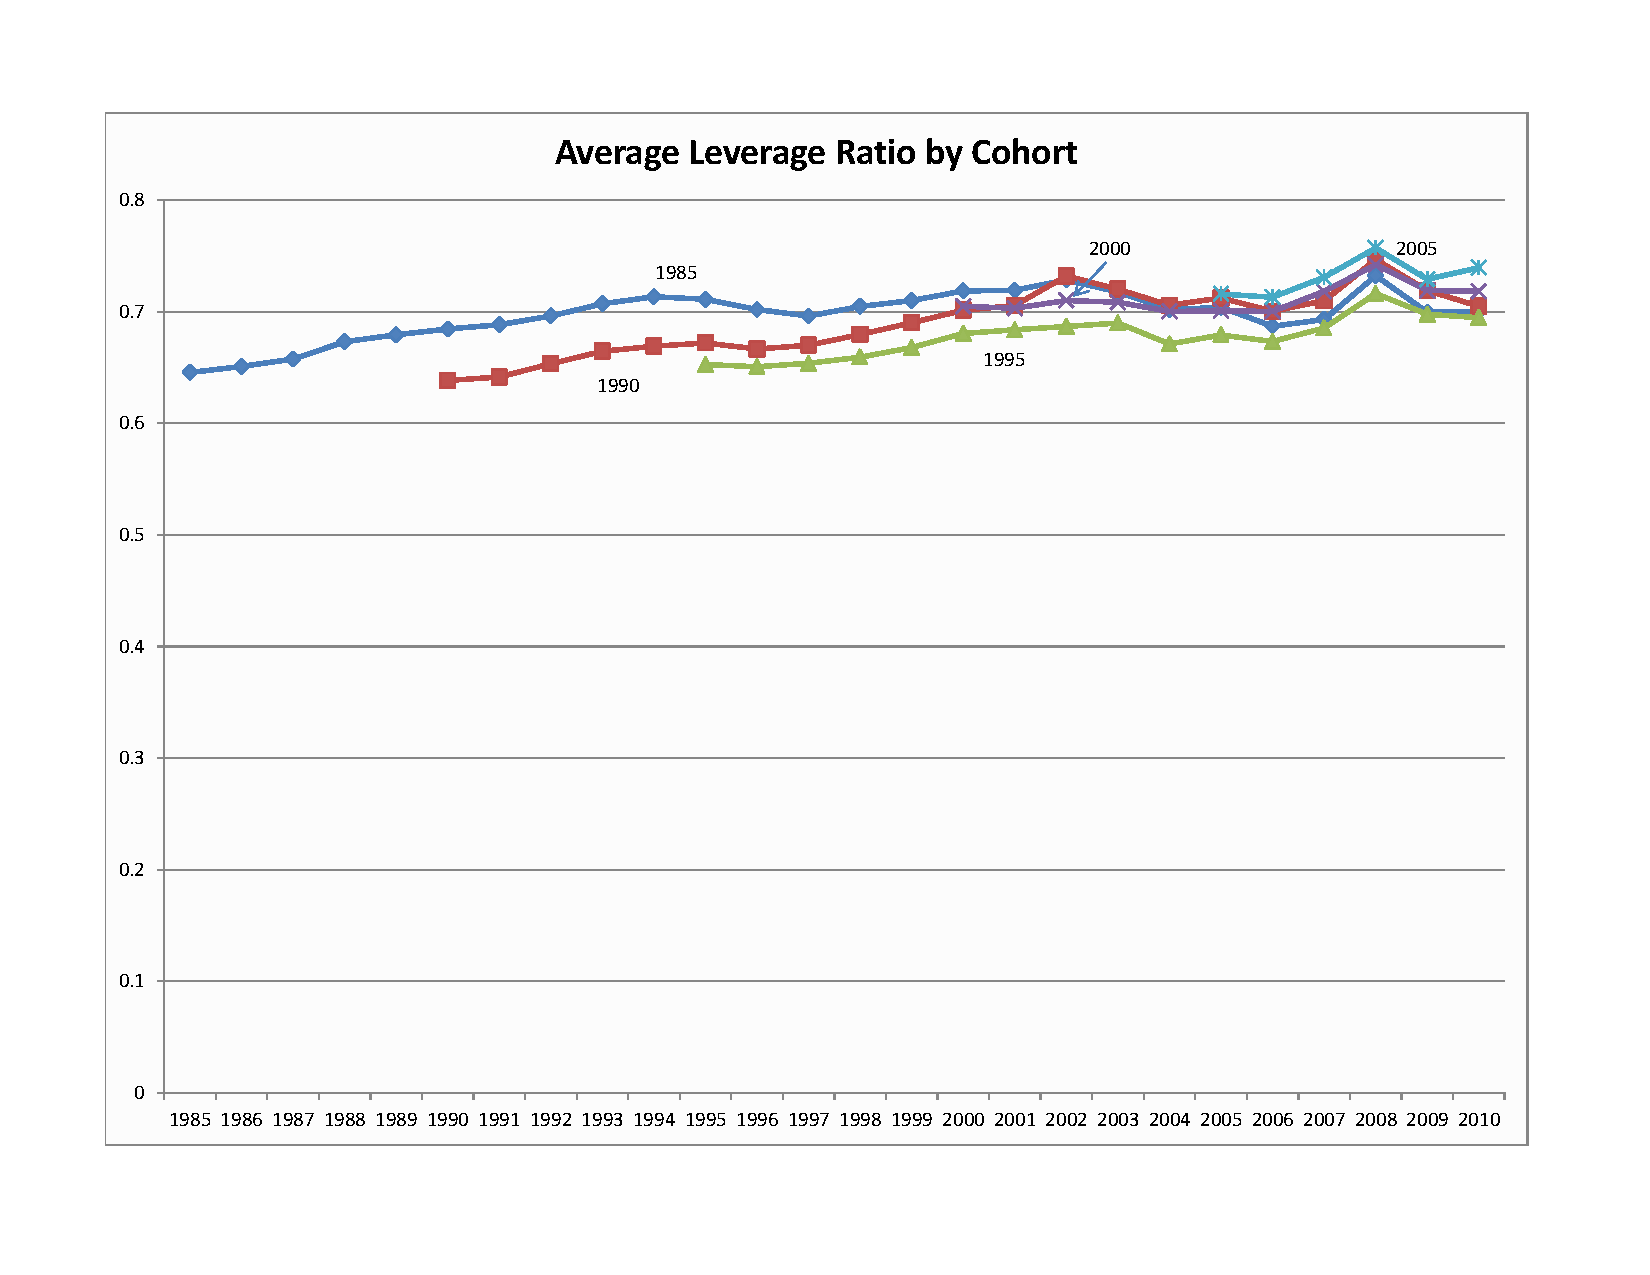
\includegraphics[page=1,width=\textwidth]{leverage_by_cohort_clr.pdf}
\hspace{-11cm}\hyperlink{app}{\beamergotobutton{Back}}}

\frame[plain,label=assets]{
\addtocounter{framenumber}{-1}
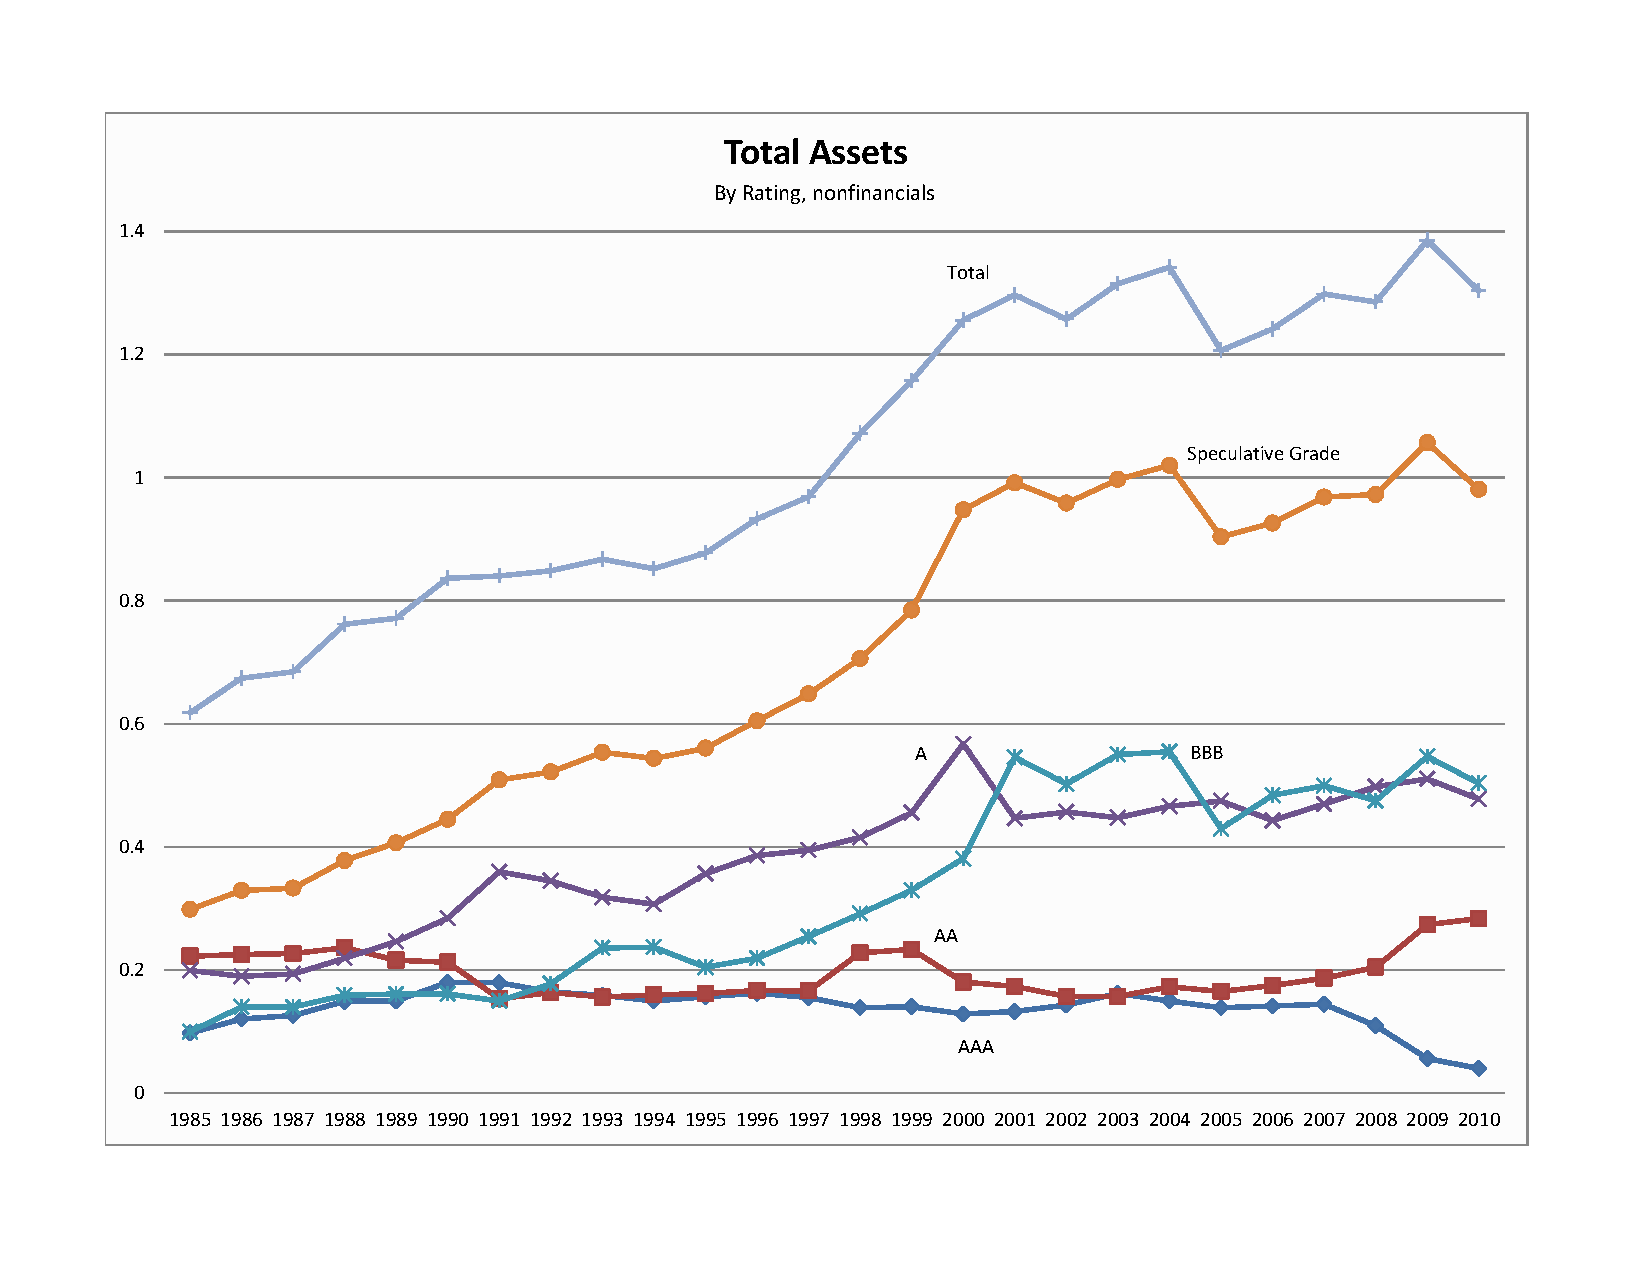
\includegraphics[page=1,width=\textwidth]{assets_nf.pdf}
\hspace{-11cm}\hyperlink{app}{\beamergotobutton{Back}}}

\frame[plain,label=cohorts]{
\addtocounter{framenumber}{-1}
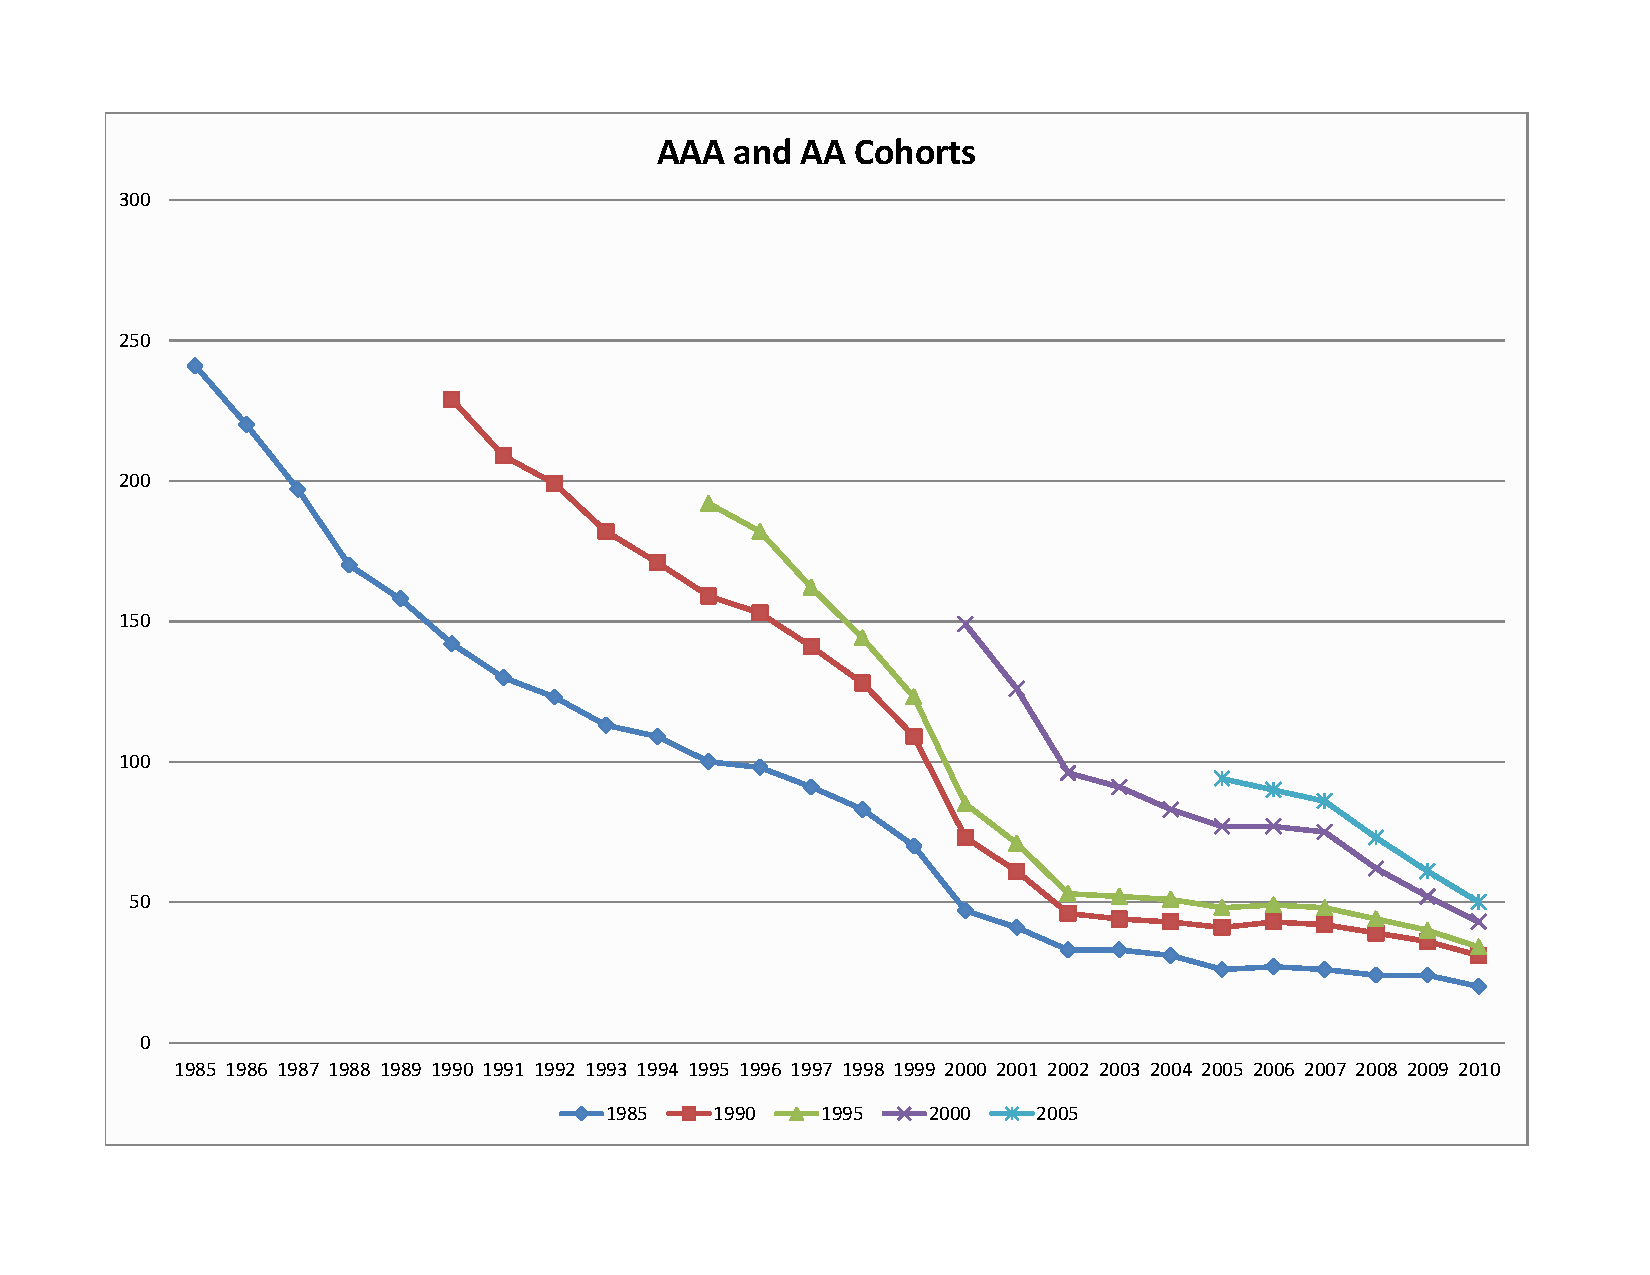
\includegraphics[page=1,width=\textwidth]{top_cohorts.pdf}
\hspace{-11cm}\hyperlink{app}{\beamergotobutton{Back}}}

% add bonds/liabilities graph?
\frame[plain,label=liab_share]{
\addtocounter{framenumber}{-1}
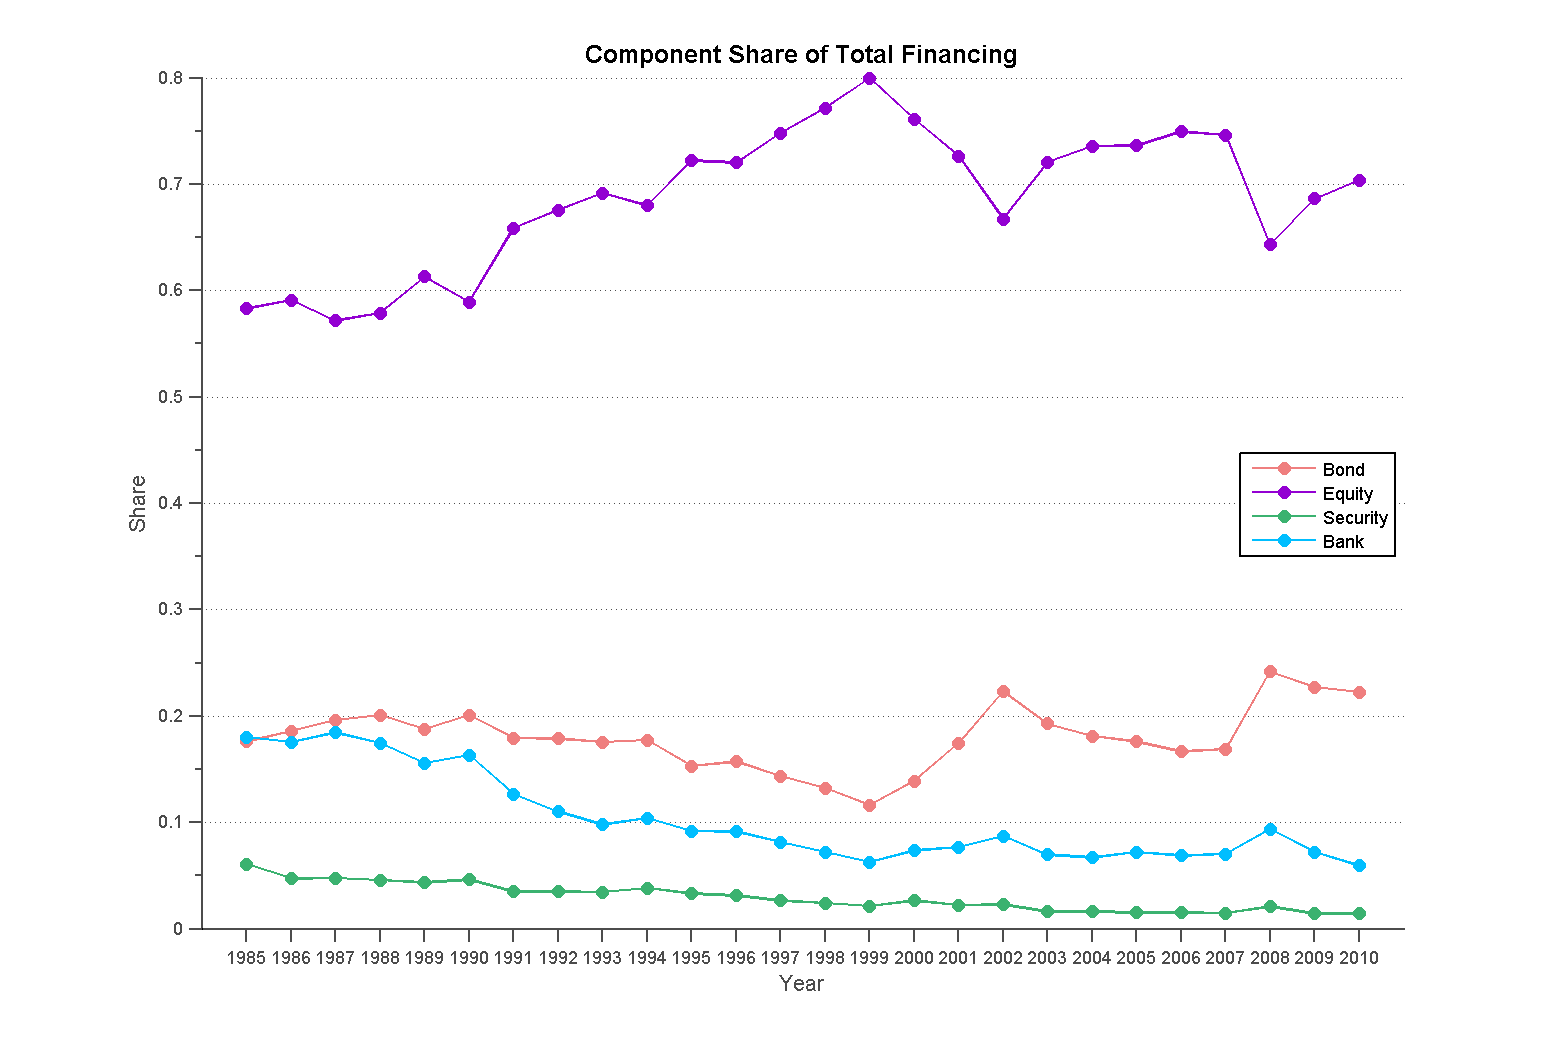
\includegraphics[page=1,width=\textwidth]{liab_share.png}
\hspace{-11cm}\hyperlink{app}{\beamergotobutton{Back}}}

\begin{frame}{CV Confidence Intervals}
\begin{itemize}
	\item Suppose r.v. $X$ is distributed log-normal with mean $\mu$ and std. dev. $\sigma$
	\item We want a confidence interval on $CV=\sqrt{Var(X)}/E(X)$
\end{itemize}
\begin{align}
E(X) & =  \exp(\mu+\frac{1}{2} \sigma^{2}) \nonumber \\
Var(X) & =  \exp(2\mu + \sigma^{2})(\exp(\sigma^{2})-1) \nonumber \\
\label{eq:cv} CV & = \sqrt{\exp(\sigma^{2})-1}
\end{align}
\end{frame}

\begin{frame}{CV Confidence Intervals}
\begin{itemize}
	\item Let $Y=\ln X$
	\item $Y$ is distributed $N(\mu,\sigma^{2})$ and the test statistic for $\sigma^{2}$ is:
\end{itemize}
\begin{align}
\frac{(n-1)s^{2}}{\sigma^{2}} & \sim \chi^{2}_{n-1} \nonumber
\end{align}
\begin{itemize}
	\item The lower and and upper bounds can be defined as follows:
\end{itemize}
\begin{align*}
a_{L}&\equiv\frac{(n-1)s^{2}}{F_{\chi^{2}}(n-1)^{-1}(1-\alpha/2)}\\
a_{U}&\equiv\frac{(n-1)s^{2}}{F_{\chi^{2}}(n-1)^{-1}(\alpha/2)}
\end{align*}
\begin{itemize}
	\item Thus, using these bounds on $\sigma^{2}$ and eq.~(\ref{eq:cv}), the following is a $1-\alpha$ confidence interval for the coeffecient of variation of $X$:
\end{itemize}
\begin{align}
\left [ \sqrt{\exp(a_{L})},\sqrt{\exp(a_{U})} \right ] \nonumber
\end{align}
\end{frame}


% Notes:
%Todo: How have bond funds changed over time?


\end{document}

